\documentclass[11pt,a4paper]{article}

\usepackage[margin=2.35cm]{geometry}
\usepackage[T1]{fontenc}
\usepackage[utf8]{inputenc}
\usepackage{lmodern}
\usepackage{microtype}
\usepackage{amsmath,amssymb,amsfonts,mathtools}
\usepackage{booktabs,longtable,array,tabularx}
\usepackage{graphicx,float,caption,subcaption}
\usepackage{xcolor}
\usepackage{listings}
\usepackage{enumitem}
\usepackage{hyperref}
\usepackage{fancyhdr}
\usepackage{lastpage}
\usepackage{url}

\definecolor{asrblue}{RGB}{25,63,104}
\definecolor{codebg}{RGB}{247,248,250}
\hypersetup{colorlinks=true,linkcolor=asrblue,citecolor=asrblue,urlcolor=asrblue,pdftitle={ASRQuant: From Scientific Literature to Auditable Quantitative Decisions and Algorithmic Trading}}
\pagestyle{fancy}
\fancyhf{}
\lhead{ASRQuant literature-to-decision laboratory}
\rhead{Alpha Stochastic Research}
\cfoot{\thepage\ of \pageref{LastPage}}
\setlength{\headheight}{14pt}
\setlist{nosep}
\captionsetup{font=small,labelfont=bf}

\lstset{
  basicstyle=\ttfamily\small,
  backgroundcolor=\color{codebg},
  frame=single,
  rulecolor=\color{black!15},
  breaklines=true,
  showstringspaces=false,
  columns=fullflexible,
  language=Python,
  keywordstyle=\color{asrblue}\bfseries,
  commentstyle=\color{black!55}
}

\newcommand{\pkg}{\texttt{ASRQuant}}
\newcommand{\R}{\mathbb{R}}
\newcommand{\E}{\mathbb{E}}
\newcommand{\Var}{\operatorname{Var}}
\newcommand{\Cov}{\operatorname{Cov}}
\newcommand{\VaR}{\operatorname{VaR}}
\newcommand{\ES}{\operatorname{ES}}

\title{\textbf{ASRQuant: From Scientific Literature to Auditable Quantitative Decisions and Algorithmic Trading}\\
\large A Unified Python Laboratory for Hypothesis Discovery, Data, Modelling, Backtesting, Robustness, and Paper Execution}
\author{Alpha Kabinet TOURE\\
Alpha Stochastic Research\\
\texttt{research@asr-lab.online}}
\date{Manuscript v0.1.0 --- ASRQuant 1.0.0 --- August 10, 2026}

\begin{document}
\maketitle

\begin{abstract}
Quantitative-finance research often begins in scientific papers but becomes fragmented when researchers manually translate claims into data requirements, features, signals, portfolios, backtests, robustness checks, and deployment decisions. This fragmentation weakens provenance: the final strategy may no longer retain the exact paper page, hypothesis statement, information lag, transformation, execution contract, or decision rule that produced it. We introduce \pkg, an open-source Python framework that connects scientific-paper ingestion, corpus-relative hypothesis discovery, explicit data planning, leakage-aware features, signal and portfolio construction, robust econometric testing, stochastic simulation, derivative and fixed-income analytics, auditable backtesting, multidimensional visualization, decision governance, and order-level paper trading through a one-import public interface. Software release 1.0.0 parses text-based PDF papers with page-level citations, preserves source-linked hypotheses in a stateful \texttt{ResearchProject}, and exposes common modelling tasks through compact entry points such as \texttt{asr.fit}, \texttt{asr.simulate}, \texttt{asr.price\_option}, \texttt{asr.visualize}, and \texttt{asr.open\_lab}. The quantitative layer includes seven core stochastic-process families, universal Monte Carlo estimators, martingale diagnostics, closed-form and numerical derivative pricing, econometrics, leakage-aware machine learning, portfolio and risk analytics, fixed income, implementation audits, and 102 module-level public visualization functions in addition to result-object plotting methods. The paper-trading layer converts target weights into orders and fills while enforcing leverage, position, turnover, cash, short-selling, commission, slippage, partial-fill, and drawdown controls. Live-capable broker primitives are separated from the research workflow and remain fail-closed unless deployment authorization is explicitly supplied. The release is validated by an automated test suite that includes a dedicated paper-contract group executing the appendix workflows and capability claims. ASRQuant remains research software: automated extraction does not establish causality or global novelty, backtests do not guarantee future profitability, and a software release is not itself authorization to deploy capital.
\end{abstract}

\noindent\textbf{Keywords:} quantitative finance; scientific literature; hypothesis discovery; economic hypotheses; stochastic processes; Monte Carlo; martingales; derivative pricing; econometrics; machine learning; backtesting; robustness; algorithmic trading; paper trading; reproducibility; Python.

\tableofcontents
\newpage

\section{Introduction}

Historical simulation is the central experimental instrument of systematic investment research. A strategy is transformed into positions, positions interact with realized returns, costs reduce gross performance, and a collection of statistics and visual diagnostics is used to judge whether the result is economically and statistically credible. The apparent simplicity of this workflow conceals many implementation choices. A signal observed at the close of day $t$ may be applied to the return from $t-1$ to $t$, to the return from $t$ to $t+1$, or to an execution price at the next open. Portfolio weights may be interpreted as pre-trade or post-trade weights. Missing observations may be dropped, forward-filled, or treated as non-tradable. Turnover may be computed before or after normalization. Costs may be charged once per rebalance, per side, or as a nonlinear function of traded notional. Each choice can alter the result even if the verbal strategy description is unchanged.

The statistical literature has extensively studied data snooping, multiple testing, inflated Sharpe ratios, and backtest overfitting \cite{white2000,hansen2005,bailey2014,bailey2017,harvey2016}. More recent work has isolated implementation risk: the dispersion induced by differences between software engines or conventions rather than by differences in the logical strategy \cite{yin2026}. This paper takes a software-engineering position on that problem. Instead of treating implementation choices as incidental keyword arguments scattered throughout code, \pkg represents them as a first-class, immutable, serializable contract.

The objective is not merely to provide another plotting library or another backtesting engine. The objective is to make a broad quantitative-research workflow both \emph{short to write} and \emph{difficult to misinterpret}. A minimal analysis is intentionally compact:

\begin{lstlisting}
import asrquant as asr
lab = asr.open_lab("prices.csv", date_column="Date")
result = lab.backtest("sma", fast=20, slow=100, costs_bps=5)
asr.save(result, "dashboard.png", kind="dashboard")
asr.report(result, "report.html")
\end{lstlisting}

However, the apparent simplicity is backed by an explicit default contract: one-bar execution delay, positive-price validation, deterministic weight alignment, leverage enforcement, transparent turnover, explicit basis-point costs, and a machine-readable experiment fingerprint. The user can override these choices, but the choices remain inspectable.

\subsection{Research question}

The central research question is:

\begin{quote}
Can a unified quantitative-finance library connect scientific literature to auditable quantitative decisions and paper execution in a few lines of code while preserving source provenance, explicit chronology, reproducibility, statistical discipline, and broad visual coverage?
\end{quote}

The software and empirical evaluation address six subsidiary questions:

\begin{enumerate}
  \item Can backtest semantics be represented in a compact contract that is both human-readable and machine-verifiable?
  \item Can one high-level API cover market data, performance, risk, regression, portfolio, derivatives, machine learning, microstructure, and multidimensional parameter analysis through two-axis surfaces, slices, and animations without forcing the user to rewrite common formulas?
  \item Can implementation sensitivity be surfaced as a standard output rather than an optional afterthought?
  \item Can this functionality remain computationally practical on medium-scale research panels?
  \item Can source-linked hypotheses and literature gaps be represented without making unsupported claims of global novelty?
  \item Can research evidence be converted into a governed decision and order-level paper-trading record without silently authorizing live execution?
\end{enumerate}

\subsection{Contributions}

The release makes the following contributions.

\begin{enumerate}
  \item \textbf{A source-linked scientific-literature layer.} Text-based PDF papers are parsed page by page; extracted hypotheses retain source excerpts, page numbers, paper fingerprints, confidence scores, and corpus-relative novelty labels.
  \item \textbf{A literature-to-decision research state machine.} A \texttt{ResearchProject} records the hypothesis, data plan, features, signal, portfolio, econometric test, backtest, robustness results, decision, paper-trading session, and chronological workflow history.
  \item \textbf{An end-to-end quantitative research object.} \texttt{QuantLab} creates one path from files or remote providers to transformations, models, backtests, audits, figures, and reports.
  \item \textbf{A provider-neutral data layer.} The same tabular contract accepts CSV and JSON in the base installation, SQL through an explicit connection, Parquet/Excel/Feather through the optional data extra, and Alpha Vantage, Binance, FRED, and optional Yahoo provider adapters, with explicit field selection and source metadata.
  \item \textbf{A stochastic-process and Monte Carlo laboratory.} Seven process families, reproducible random seeds, antithetic sampling, pricing standard errors, and confidence intervals are exposed through a common result object.
  \item \textbf{Integrated derivative analytics.} Black--Scholes--Merton, Bachelier, Black--76, CRR trees, implied volatility, analytic and numerical Greeks, European Monte Carlo, and arithmetic-average Asian Monte Carlo are available without external pricing code.
  \item \textbf{Finite-sample martingale diagnostics.} Discounting, mean-increment tests, HAC predictive regressions, and Ljung--Box diagnostics make the martingale hypothesis inspectable while explicitly avoiding the false claim that finite data can prove it.
  \item \textbf{A specification-first backtest contract.} Execution delay, rebalancing, leverage, missing-data policy, annualization, financing rate, and costs are encoded in an immutable \texttt{BacktestSpec}.
  \item \textbf{Econometrics and leakage-aware machine learning.} Robust and rolling OLS, quantile and polynomial regression, regularization, logistic and factor models, cointegration, Granger-predictive tests, ARIMA, VAR, technical features, forward targets, and chronological walk-forward evaluation share aligned outputs.
  \item \textbf{Broad risk, allocation, volatility, and fixed-income coverage.} The package includes historical and parametric tail risk, drawdown duration, CDaR, covariance shrinkage, maximum diversification, HRP, Black--Litterman, realized and range-based volatility, GARCH integration, bond pricing, yield, duration, convexity, and par-curve bootstrapping on an explicit complete coupon grid.
  \item \textbf{Implementation-risk auditing and reproducibility.} Alternative delays, costs, and rebalance rules generate uncertainty intervals and conclusion-stability statistics; deterministic fingerprints and manifests record the experiment.
  \item \textbf{A multidimensional parameter explorer.} Any scalar-valued experiment on a finite grid can be reduced to two selected surface axes; any number of remaining numeric or categorical parameters can be fixed or flattened into reproducible animation frames, with dotted-path metric extraction, parallel evaluation, failure metadata, best-point extraction, and HTML/GIF/MP4 export.
  \item \textbf{A tested visualization system.} More than 100 public visualization functions and result-object plotting methods cover market data, stochastic paths, martingales, regressions, ML, risk, portfolios, derivatives, microstructure, heatmaps, contours, interactive 3D surfaces, and parameter animations.
  \item \textbf{A broker-neutral paper-execution layer.} Target weights are translated into orders, fills, cash, positions, realized weights, and risk events under explicit leverage, position, turnover, order-notional, cash, short-selling, commission, slippage, partial-fill, and drawdown controls.
\end{enumerate}

\section{Related Work}

\subsection{Backtesting systems}

Python backtesting systems occupy several design points. Event-driven frameworks model orders, fills, and broker interactions in detail. Vectorized frameworks represent signals and positions as arrays, enabling fast parameter sweeps. Performance-analysis packages produce tear sheets from precomputed returns. Examples include Backtrader, Zipline, backtesting.py, vectorbt, pyfolio, empyrical, and QuantStats. These projects have substantially lowered the barrier to quantitative experimentation. Nevertheless, they generally specialize in one layer of the workflow: execution simulation, analytics, or reporting. \pkg adopts a complementary position. It provides a lightweight reference backtester, but its primary abstraction is the experiment contract and the consistent propagation of that contract into audit outputs and reports.

Vectorized computation is particularly appropriate when the strategy can be represented as target weights over a common time index. Array-oriented systems can evaluate many assets or parameter configurations efficiently, while event-driven systems are more natural for intrabar order logic, partial fills, and exchange-specific mechanics. \pkg therefore does not claim to replace a production execution simulator. It deliberately targets research-grade daily or bar-based portfolio experiments in which signal timestamps and target weights can be made explicit.

\subsection{Performance and risk analytics}

The Sharpe ratio and related risk-adjusted statistics are standard in investment evaluation \cite{sharpe1966}. Their interpretation requires care under serial dependence and non-normality \cite{lo2002}. Drawdown, Sortino, Calmar, Omega, Value at Risk, and Expected Shortfall provide complementary views of the return distribution and path. Existing analytics packages automate many of these calculations. \pkg integrates these measures with turnover, costs, implementation warnings, and the exact specification fingerprint used to produce them.

\subsection{Backtest overfitting and multiple testing}

White's Reality Check and Hansen's Superior Predictive Ability test address data-snooping bias when many models are compared \cite{white2000,hansen2005}. The Deflated Sharpe Ratio corrects an observed Sharpe ratio for multiple selection and non-normal returns \cite{bailey2014}. The Probability of Backtest Overfitting formalizes the likelihood that a selected in-sample configuration underperforms out of sample \cite{bailey2017}. Harvey, Liu, and Zhu show that conventional significance thresholds are too weak when hundreds of factors are tested \cite{harvey2016}. \pkg does not claim to fully automate all possible multiple-testing procedures in software release 1.0.0, but it includes probabilistic and deflated Sharpe diagnostics, block bootstrap confidence intervals, permutation tests, and Benjamini--Hochberg false-discovery-rate control.

\subsection{Implementation risk and design uncertainty}

Yin et al. distinguish statistical overfitting from engine-level disagreement and propose metrics for implementation risk \cite{yin2026}. Their results show that transaction-cost details can create structured divergence across engines. Related 2026 work studies design uncertainty across implementation choices \cite{battistella2026}. \pkg operationalizes this concern at the API level: users can call \texttt{lab.audit(...)} on the same target weights and inspect the distribution of performance across specified conventions. We use the neutral term \emph{contract sensitivity} because the grid may contain both defensible alternatives and intentionally unrealistic diagnostics such as same-bar execution.

\subsection{Scientific Python and visualization}

The implementation builds on NumPy, pandas, SciPy, Matplotlib, Plotly, statsmodels, and scikit-learn \cite{harris2020,mckinney2010,virtanen2020,hunter2007,pedregosa2011,seabold2010}. The contribution is not a replacement for these libraries; it is a finance-specific composition layer with standardized inputs, outputs, formulas, and audit metadata.

\section{Design Principles}

\pkg follows eight design principles.

\subsection{Explicit semantics over convenient ambiguity}

A backtest that cannot state when a signal becomes tradable is incomplete. Defaults are allowed, but defaults must be documented, inspectable, and included in the experiment fingerprint.

\subsection{A short public API over duplicated notebooks}

Common formulas should not be manually reimplemented in each project. The high-level API should cover the common path, while lower-level functions remain available for specialists.

\subsection{Pandas-compatible inputs and outputs}

A \texttt{Series} or \texttt{DataFrame} with a time index is the standard interchange format. This choice facilitates integration with data vendors, statistical packages, and notebooks.

\subsection{Deterministic transformations}

Given identical data, configuration, and package version, the engine should produce identical results. Random procedures require an explicit random seed.

\subsection{No hidden forward filling}

Price returns are computed with \texttt{fill\_method=None}. Missing-data policies are selected before return calculation. This avoids silently creating zero returns across gaps.

\subsection{Warnings should be structural}

Same-bar execution is not forbidden because it can be useful as a diagnostic or for signals known before the bar begins. It is, however, marked in the result metadata and HTML report as a potential look-ahead risk.

\subsection{Visualization must preserve the underlying object}

Plot functions return figure objects rather than forcing display. Researchers can save, modify, test, or embed the figures.

\subsection{Research scope must remain honest}

The package is a research framework. Software release 1.0.0 models market, limit, stop, and stop-limit order states and configurable partial fills in a deterministic paper broker. A separate guarded live module can connect an explicitly configured broker adapter, but live authorization is fail-closed and is not implied by a successful backtest or by installation of the package. The framework does not model exchange queue priority, venue latency, market halts, borrow recalls, corporate-action databases, or full broker-specific market microstructure.

\section{Formal Backtest Contract}

\subsection{Market data and returns}

Let $P_{t,i}>0$ be the observed price of asset $i\in\{1,\ldots,N\}$ at timestamp $t\in\{0,\ldots,T\}$. Simple returns are

\begin{equation}
 r_{t,i}=\frac{P_{t,i}}{P_{t-1,i}}-1,
 \qquad t=1,\ldots,T.
\end{equation}

No return is defined across an unresolved missing observation. The data policy is one of:

\begin{enumerate}
  \item \texttt{raise}: reject any missing price;
  \item \texttt{drop}: retain only rows complete across the selected assets;
  \item \texttt{ffill}: forward-fill first, then remove unresolved leading gaps.
\end{enumerate}

The policy is part of the contract and therefore part of the specification fingerprint.

\subsection{Target and effective weights}

Let $z_{t,i}$ be the target weight produced by the strategy at timestamp $t$. Let $\delta\in\{0,1,2,\ldots\}$ denote the execution delay in bars. Effective weights for the return ending at $t$ are

\begin{equation}
 w_{t,i}=z_{t-\delta,i},
\end{equation}

with unavailable pre-sample targets set to zero. Under the default $\delta=1$, a signal formed at time $t$ affects the next bar's return. Setting $\delta=0$ applies the current target to the current return and must be justified by the information timestamp.

\subsection{Constraints}

For maximum absolute asset weight $u>0$ and maximum gross leverage $L>0$, raw targets are clipped and rescaled so that

\begin{equation}
 |w_{t,i}|\leq u,
 \qquad
 \sum_{i=1}^{N}|w_{t,i}|\leq L.
\end{equation}

If \texttt{long\_only=True}, negative targets are set to zero before leverage normalization. This is a deterministic projection, not a general constrained optimizer.

\subsection{Turnover}

One-way portfolio turnover is defined as

\begin{equation}
 \tau_t=\sum_{i=1}^{N}|w_{t,i}-w_{t-1,i}|.
\end{equation}

This convention counts a complete rotation from one fully invested asset to another as turnover $2$. Because industry turnover definitions vary, the report labels the quantity explicitly as fraction of net asset value traded.

\subsection{Transaction and financing costs}

Let $b$ be the sum of commission, spread, and slippage rates in basis points. Let $\kappa\geq 0$ and $\gamma\geq 1$ parameterize nonlinear market impact. Let $q$ be the annualized short-borrow rate in basis points and $A$ the annualization factor. The period cost is

\begin{equation}
 C_t = \frac{b}{10^4}\tau_t
      +\kappa\tau_t^{\gamma}
      +\frac{q}{10^4 A}\sum_{i=1}^{N}\max(-w_{t,i},0).
\end{equation}

This model is intentionally transparent. It is not a substitute for an empirically calibrated execution model based on volume, volatility, spread, and participation rate. Market-impact theory motivates nonlinear cost functions \cite{almgren2001}, but calibration remains asset- and venue-specific.

\subsection{Cash and portfolio return}

The residual cash weight is

\begin{equation}
 c_t = 1-\sum_{i=1}^{N}w_{t,i}.
\end{equation}

For annualized risk-free rate $r_f$, gross and net portfolio returns are

\begin{align}
 R_t^{\mathrm{gross}} &= \sum_{i=1}^{N}w_{t,i}r_{t,i},\\
 R_t^{\mathrm{net}} &= R_t^{\mathrm{gross}} + c_t\frac{r_f}{A} - C_t.
\end{align}

Equity evolves from initial capital $V_0$ according to

\begin{equation}
 V_t=V_0\prod_{s=1}^{t}(1+R_s^{\mathrm{net}}).
\end{equation}

\subsection{Rebalancing}

A target panel can be applied every bar or sampled at a calendar rule such as weekly, monthly, or quarterly. After sampling, targets are carried forward until the next rebalance. The distinction between signal refresh and execution refresh is important: a daily signal evaluated under monthly rebalancing is not equivalent to a genuinely monthly signal.

\subsection{Contract fingerprint}

The specification is serialized as sorted JSON and hashed with SHA-256. The data frame is separately fingerprinted from values, timestamps, and column names. The experiment identifier combines both fingerprints. The hash is not a proof of data correctness; it is an identity check that detects changes to the analyzed object or contract.

\section{Implementation-Sensitivity Diagnostics}

Let $\mathcal{C}=\{c_1,\ldots,c_K\}$ be a set of backtest contracts applied to the same prices and logical target weights. For a metric $m$, write $\theta_m(c_k)$ for the result under contract $c_k$.

\subsection{Implementation uncertainty interval}

\begin{equation}
 \operatorname{IUI}_m =
 \left[
 \min_{c\in\mathcal{C}}\theta_m(c),
 \max_{c\in\mathcal{C}}\theta_m(c)
 \right].
\end{equation}

This interval is descriptive. It does not have a sampling-probability interpretation unless the contract set itself is generated from a probabilistic design.

\subsection{Engine sensitivity}

\begin{equation}
 \operatorname{ES}_m =
 \max_{c\in\mathcal{C}}\theta_m(c)
 -\min_{c\in\mathcal{C}}\theta_m(c).
\end{equation}

A large value indicates that the reported metric is highly conditional on implementation choices.

\subsection{Conclusion stability index}

For a directional conclusion based on total return, define

\begin{equation}
 \operatorname{CSI}=
 \left|
 \frac{1}{K}\sum_{k=1}^{K}\operatorname{sign}\left(\theta_{\mathrm{TR}}(c_k)\right)
 \right|.
\end{equation}

The index equals one when all contracts agree on the sign and approaches zero when positive and negative conclusions are balanced. This simple release metric is related in spirit to conclusion-sensitivity measures in recent implementation-risk research \cite{yin2026}; future versions will support user-defined decision rules and equivalence margins.

\section{Software Architecture}

\begin{figure}[H]
\centering
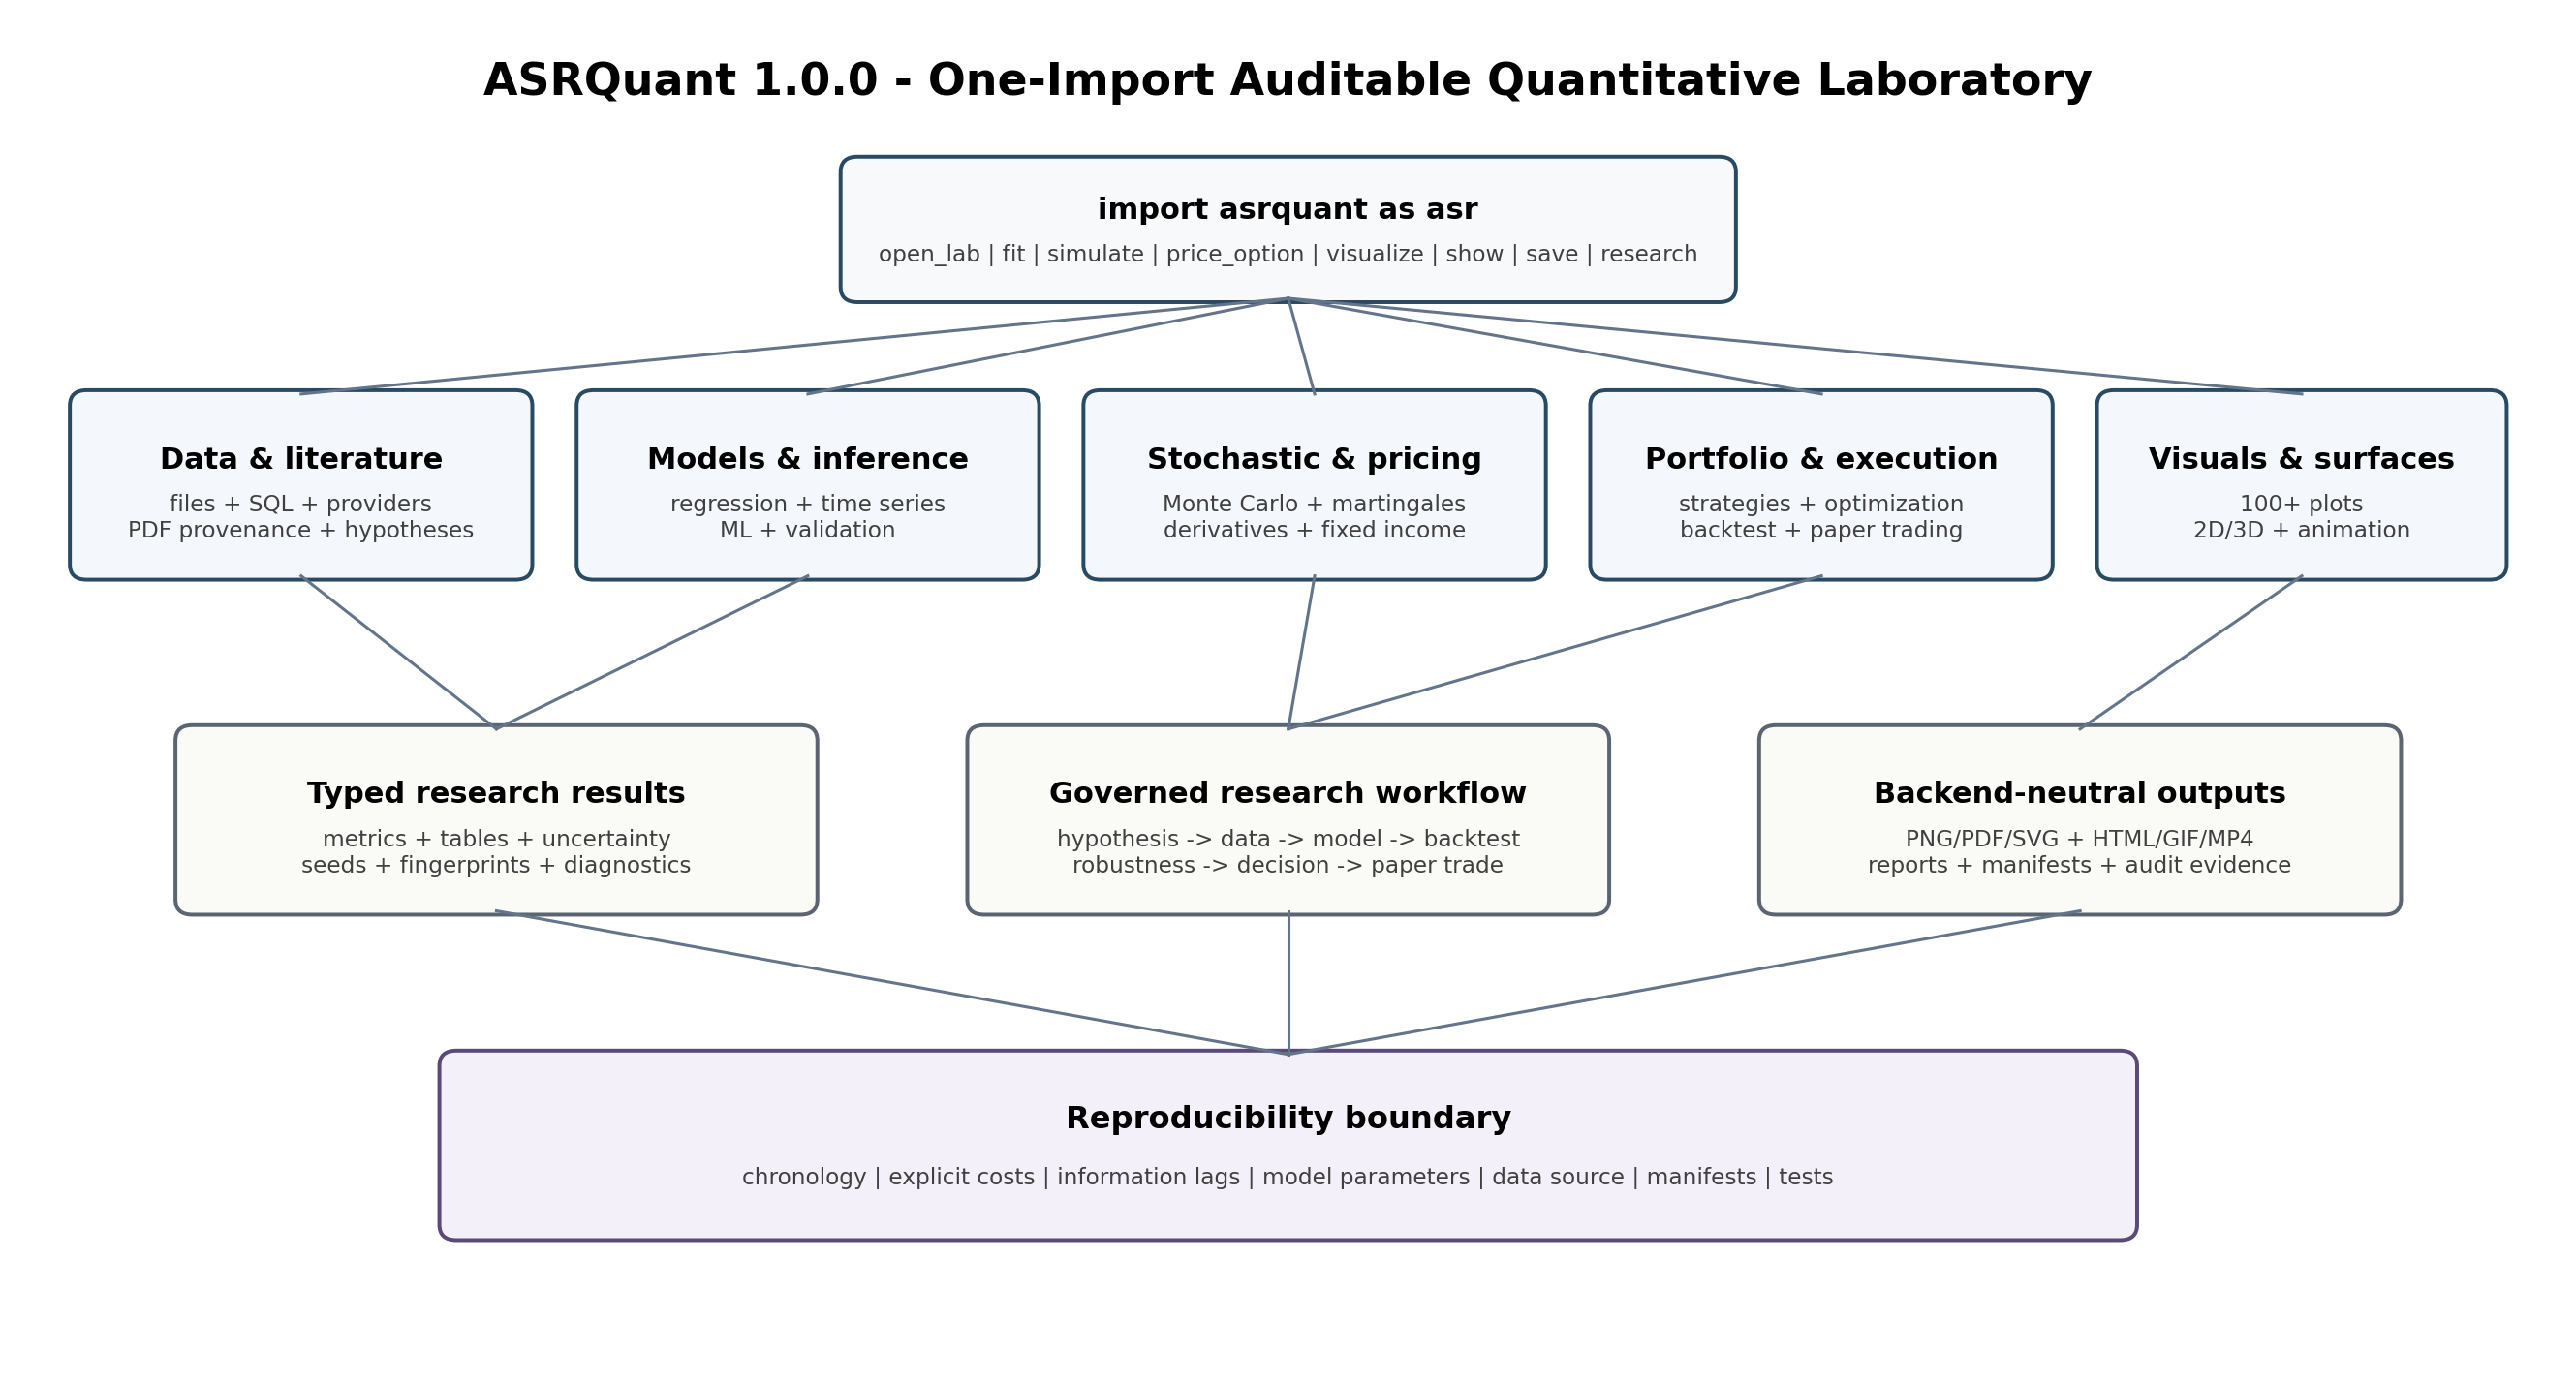
\includegraphics[width=\textwidth]{figures/asrquant_architecture_v100.png}
\caption{ASRQuant 1.0.0 architecture. The public API is intentionally short, but each output retains the data source, model parameters, research contract, and uncertainty information required for audit.}
\label{fig:architecture}
\end{figure}

\begin{longtable}{p{0.39\textwidth}p{0.55\textwidth}}
\caption{Principal modules in software release 1.0.0.}\label{tab:modules}\\
\toprule
Module & Responsibility \\
\midrule
\endfirsthead
\toprule
Module & Responsibility \\
\midrule
\endhead
\texttt{easy.py}, \texttt{models.py}, \texttt{math.py} & One-import facade, backend-neutral figure handles, friendly estimator factories, model-name resolution, table constructors, and numerical helpers. \\
\texttt{api.py} & High-level \texttt{QuantLab}: files, providers, models, regression, ML, pricing, backtests, sweeps, figures, and reports. \\
\texttt{data.py}, \texttt{providers.py} & Local and SQL loading, validation, OHLCV aggregation, quality reports, fingerprints, provider adapters, and polling feeds. \\
\texttt{simulation.py}, \texttt{monte\_carlo.py}, \texttt{martingales.py} & Seven core stochastic-process families, correlated GBM, regime-switching synthetic markets, universal Monte Carlo estimators, pricing uncertainty, stationary bootstrap, and martingale diagnostics. \\
\texttt{derivatives.py}, \texttt{fixed\_income.py}, \texttt{approximation.py} & BSM, Bachelier, Black--76, CRR, implied volatility, Greeks, bond and yield analytics, par-curve bootstrap, interpolation, surrogate regression, gradients, and Hessians. \\
\texttt{statistics.py}, \texttt{machine\_learning.py} & Econometrics, inference, time-series models, feature engineering, forward targets, chronological validation, and walk-forward evaluation. \\
\texttt{strategies.py}, \texttt{backtest.py}, \texttt{audit.py}, \texttt{surfaces.py} & Nine strategy constructors, vectorized backtests, transparent costs, trade ledgers, implementation audits, parameter sweeps, N-dimensional experiment evaluation, and static/animated surfaces. \\
\texttt{literature.py}, \texttt{workflow.py}, \texttt{research.py}, \texttt{trading.py} & PDF provenance, hypothesis registry, research-state machine, governed decisions, market/limit/stop order primitives, deterministic paper broker, partial fills, and risk controls. \\
\texttt{metrics.py}, \texttt{volatility.py}, \texttt{optimization.py} & Performance, benchmark, drawdown, tail risk, Sharpe-quality, realized/range-based volatility, optional GARCH, covariance estimation, ERC, HRP, maximum diversification, and Black--Litterman. \\
\texttt{production.py}, \texttt{audit\_store.py}, \texttt{live.py} & Fail-closed deployment evidence, tamper-evident SQLite audit storage, reconciliation, kill-switch and pre-trade risk primitives, and guarded broker adapters kept separate from research authorization. \\
\texttt{report.py}, \texttt{provenance.py}, \texttt{viz/*} & Portable reports, manifests, and 102 module-level public visualization functions plus result-object plotting methods. \\
\bottomrule
\end{longtable}

The architecture separates the public research contract from implementation engines. The recommended user surface is a single import, \texttt{import asrquant as asr}. The \texttt{models} namespace creates validated estimators, \texttt{math} provides numerical and distribution helpers, and \texttt{visualize}, \texttt{show}, and \texttt{save} wrap static and interactive rendering behind a backend-neutral handle. Calculations return scalars, compatible tables, or typed result containers. Mature numerical, econometric, machine-learning, and visualization libraries remain internal because reimplementing them would increase numerical and maintenance risk; ordinary workflows do not import or orchestrate them directly. Network access is isolated in provider adapters; no import or model operation silently performs a remote request. Remote acquisition and near-real-time polling are data functions only and cannot place orders.

\section{Visualization Taxonomy}

Software release 1.0.0 contains 102 module-level public visualization functions, excluding private helpers, plus result-object plotting methods. Table~\ref{tab:viz} summarizes the coverage.

\begin{longtable}{p{0.18\textwidth}p{0.74\textwidth}}
\caption{Visualization coverage.}\label{tab:viz}\\
\toprule
Category & Included diagnostics \\
\midrule
\endfirsthead
\toprule
Category & Included diagnostics \\
\midrule
\endhead
Market data & Prices, normalized prices, log scale, returns, cumulative returns, dependency-light candlesticks, rolling mean and volatility, distribution with KDE and normal overlay, ECDF, Q--Q, box and violin plots, ACF, PACF, static and rolling correlation, monthly and daily-calendar heatmaps, scatter matrix. \\
Performance & Equity, equity plus drawdown, dashboard, rolling Sharpe and Sortino, annual and monthly returns, turnover, costs, gross/net exposure, weights, return contributions, benchmark comparison, rebalance-bar returns. \\
Risk & Historical, Gaussian, and Cornish--Fisher VaR; Expected Shortfall; rolling tail risk; empirical loss tails; CDaR; drawdowns; stress bars; sensitivity heatmaps; Monte Carlo fans; contract-audit plots. \\
Stochastic processes & Path ensembles, uncertainty fans, terminal distributions, Monte Carlo convergence, and martingale diagnostic panels. \\
Regression & Regression scatter, actual versus fitted, residual four-panel diagnostics, coefficient intervals, rolling coefficients, factor-exposure heatmaps. \\
Portfolio & Efficient-frontier cloud, allocation pie, risk contributions, correlation network, weights heatmap. \\
Derivatives & Payoff diagrams, BSM/Bachelier comparisons, option value curves, Greek curves, implied-volatility surfaces, Greek surfaces, Monte Carlo convergence, and yield curves. \\
Machine learning & Feature importance, prediction paths, residuals, ROC, confusion matrix, calibration, regime probabilities. \\
Microstructure & Bid--ask spread, volume profile, order-book depth, slippage curve, trade timeline. \\
General 2D/3D & Generic response surfaces, parameter heatmaps, contour maps, interactive Plotly surfaces, multi-parameter frame sliders, stable-scale animations, and GIF/MP4 export. \\
\bottomrule
\end{longtable}

The goal is not to assert that every plot should be used in every paper. The goal is to make standard diagnostics easy enough that researchers are less tempted to omit them due to implementation cost.

\section{Performance and Risk Metrics}

For return series $R_1,\ldots,R_T$ and annualization factor $A$, the annualized arithmetic volatility is

\begin{equation}
 \widehat{\sigma}_{A}=\sqrt{A}\,\widehat{\sigma}(R).
\end{equation}

The compound annual growth rate is

\begin{equation}
 \operatorname{CAGR}=\left(\prod_{t=1}^{T}(1+R_t)\right)^{A/T}-1.
\end{equation}

The annualized Sharpe ratio is

\begin{equation}
 \widehat{SR}=\sqrt{A}\,
 \frac{\overline{R}-r_f/A}{\widehat{\sigma}(R-r_f/A)}.
\end{equation}

The package reports \texttt{NaN} when volatility is numerically zero rather than returning an infinite Sharpe ratio. The Sortino ratio replaces total volatility with root-mean-square downside deviation. Maximum drawdown is computed from the running wealth maximum:

\begin{align}
 W_t &= \prod_{s=1}^{t}(1+R_s),\\
 D_t &= \frac{W_t}{\max_{u\leq t}W_u}-1,\\
 \operatorname{MDD} &= \min_t D_t.
\end{align}

Historical Value at Risk and Expected Shortfall at confidence level $\alpha$ are

\begin{align}
 \VaR_{\alpha} &= -Q_{1-\alpha}(R),\\
 \ES_{\alpha} &= -\E\left[R\mid R\leq Q_{1-\alpha}(R)\right].
\end{align}

The metrics table also includes Calmar, Omega, ulcer index, tail ratio, hit rate, profit factor, skewness, excess kurtosis, probabilistic Sharpe ratio, average turnover, annual turnover, and optional benchmark alpha, beta, tracking error, and information ratio.

\section{Regression and Statistical Diagnostics}

\subsection{OLS and robust covariance}

For dependent variable $y$ and regressor matrix $X$, \pkg estimates

\begin{equation}
 y=X\beta+\varepsilon
\end{equation}

by ordinary least squares. The default covariance estimator is heteroskedasticity-and-autocorrelation consistent (HAC/Newey--West style), with an automatically selected lag proportional to $T^{1/4}$ unless the user specifies it. HC0--HC3 and classical covariance are also available. Returned diagnostics include $R^2$, adjusted $R^2$, Durbin--Watson, Jarque--Bera, Ljung--Box, Breusch--Pagan, and White-test p-values.

\subsection{Rolling regression}

Rolling OLS exposes time-varying factor loadings. For window $h$, coefficients at time $t$ solve

\begin{equation}
 \widehat{\beta}_t=\arg\min_{\beta}
 \sum_{s=t-h+1}^{t}(y_s-X_s\beta)^2.
\end{equation}

The visualization layer displays coefficient paths and factor-exposure heatmaps.

\subsection{Stationarity tests}

The Augmented Dickey--Fuller and KPSS tests are reported together because their null hypotheses differ. The software does not convert the pair into an automatic stationarity verdict; interpretation remains the user's responsibility.

\subsection{Dependent-data bootstrap}

A moving-block bootstrap resamples contiguous blocks, preserving local dependence better than an i.i.d. bootstrap. The default block length is proportional to $T^{1/3}$. The function returns the point estimate, percentile confidence bounds, and bootstrap standard error.

\subsection{Multiple testing}

Benjamini--Hochberg adjusted p-values are provided for false-discovery-rate control. The approximate Deflated Sharpe Ratio uses the expected maximum Sharpe under a specified number of trials and then evaluates a probabilistic Sharpe statistic. This is a research diagnostic; a complete trial ledger remains necessary for credible interpretation.

\subsection{Extended regression and time-series models}

Quantile regression estimates a conditional quantile $Q_\tau(y\mid X)=X\beta_\tau$ and is useful when predictor relationships differ across the return distribution. Polynomial transformations allow controlled nonlinear terms. Ridge, Lasso, and Elastic Net are implemented through standardized scikit-learn pipelines. Binary logistic regression returns probabilities, robust coefficient intervals, pseudo-$R^2$, AIC, and BIC. Factor regression applies the same HAC infrastructure to excess returns. Engle--Granger cointegration, Granger-predictive tests, ARIMA, and vector autoregression are exposed as explicit models; the term ``Granger causality'' is interpreted only as incremental predictability and not as structural causation.

\subsection{Leakage-aware machine learning}

For price $P_t$ and horizon $h$, the default regression target is
\begin{equation}
 y_t=\frac{P_{t+h}}{P_t}-1,
\end{equation}
with the last $h$ observations left undefined. Feature constructors generate only explicit lags and rolling statistics; they never backward-fill future information. Each walk-forward fold fits a fresh estimator clone on chronological training data, optionally inserts a gap, and evaluates regression with RMSE, MAE, and $R^2$ or classification with accuracy, ROC AUC, and log loss. This design cannot detect every semantic leak, but it prevents random temporal shuffling and accidental estimator reuse across folds.

\section{Time-Aware Validation and Leakage Controls}

Random train/test splitting is generally inappropriate for autocorrelated financial time series. \pkg therefore provides ordered walk-forward splits with fixed or expanding training windows. If $I_k^{\mathrm{train}}$ and $I_k^{\mathrm{test}}$ denote the $k$th split, the invariant is

\begin{equation}
 \max I_k^{\mathrm{train}} < \min I_k^{\mathrm{test}}.
\end{equation}

Purged K-fold splitting removes observations near the test interval and applies an optional embargo after the interval. This reduces overlap when labels or features span multiple periods. A heuristic leakage report also compares signal correlations with same-bar and next-bar returns and checks index ordering. These checks cannot prove absence of leakage. Point-in-time source validation and feature-specific availability timestamps remain essential.

\section{Data Ingestion and Near-Real-Time Feeds}

\pkg accepts a pandas Series or DataFrame directly and provides constructors for CSV, Parquet, Excel, JSON, Feather, and SQL. The local-file contract is:

\begin{lstlisting}
import asrquant as asr
lab = asr.QuantLab.from_csv(
    "prices.csv", date_column="Date",
    columns=["SPY", "TLT", "GLD"]
)
print(lab.quality)
\end{lstlisting}

Provider adapters expose one method, \texttt{history(symbol, **kwargs)}, and normalize provider-specific responses into time-indexed pandas tables. Software release 1.0.0 includes Alpha Vantage equities/intraday data, public Binance Spot candles, FRED macroeconomic series, and optional Yahoo downloads. Multiple symbols are aligned by timestamp and field. A \texttt{PollingFeed} yields the latest observation at an explicit interval for notebooks and dashboards. It is intentionally not a WebSocket order-management or brokerage component. Provider availability, entitlements, redistribution rights, rate limits, timestamp semantics, and real-time status remain properties of the upstream service and must be recorded by the researcher.


\section{Scientific Literature and Hypothesis Provenance}

Let a supplied corpus be $\mathcal{C}=\{P_1,\ldots,P_J\}$, where every paper $P_j$ is represented as a sequence of extracted pages $P_j=(p_{j1},\ldots,p_{jM_j})$. A source excerpt is the tuple
\[
e=(j,m,s),
\]
where $j$ identifies the paper, $m$ identifies the page, and $s$ is the extracted sentence. A candidate hypothesis $H_k$ stores a statement, an expected direction when recoverable, a confidence score, and a nonempty evidence set $E_k$ of such tuples. The page coordinate is preserved throughout reporting so that a researcher can inspect the original context rather than accepting a detached generated summary.

The default extractor is deterministic and conservative. It identifies hypothesis-like language, research questions, directional claims, and future-work or limitation statements. Similar candidates are grouped with transparent token overlap. A custom extractor may connect a language model, but it must return the same page-linked evidence contract. The framework does not treat generated output as evidence unless the source passage is stored.

A separate evidence-status field distinguishes passages that appear to report an empirical test, passages that explicitly state an untested gap, and passages that merely propose a relationship. These labels are triage metadata rather than final scientific judgments; the cited page remains the authoritative object for human review.

Novelty labels are defined only relative to $\mathcal{C}$. If $n_k$ is the number of distinct papers supporting candidate $H_k$, the current heuristic distinguishes established claims, replicated claims, underexplored claims, contradictory directional language, and corpus gaps. The label ``corpus-novel'' means
\[
\nexists H_{\ell}\in\mathcal{C}\setminus\{P_j\}\text{ directly matched by the supplied retrieval procedure},
\]
not that no related paper exists in the global literature. This distinction is essential because a finite local corpus cannot prove a universal negative about prior research.

Scanned PDFs with no extractable text are flagged rather than silently processed. Optical character recognition may change symbols, signs, equations, and variable names; therefore OCR must be performed and reviewed outside the default ingestion path before a scientific claim is extracted.

\section{Hypothesis-to-Decision Research Workflow}

An operational economic hypothesis is represented as
\[
H=(q,x,y,d,h,\mathcal{U},H_0,\mathcal{M},\mathcal{F}),
\]
where $q$ is the verbal claim, $x$ is the predictor, $y$ is the target, $d$ is the expected sign, $h$ is the horizon, $\mathcal{U}$ is the universe, $H_0$ is the null, $\mathcal{M}$ is the economic mechanism, and $\mathcal{F}$ is a set of falsification criteria. The object can be constructed from a paper-linked candidate or entered directly by the researcher.

A data plan maps the constructs in $H$ to proposed variables, sources, symbols, frequencies, fields, availability lags, and point-in-time requirements. Provider mappings are suggestions rather than automatic construct validation. For a variable observed or published with lag $\ell_j$, a feature transformation $g_j$ is constrained to
\[
X_{j,t}=g_j(D_{j,1:t-\ell_j}),
\]
so that the feature cannot use information unavailable at the decision timestamp. Feature specifications include raw values, differences, returns, momentum, rolling moments, z-scores, exponential averages, ranks, volatility, drawdowns, ratios, spreads, and interactions.

A signal map $\phi$ transforms the feature vector into target weights,
\[
w_t^{\star}=\phi(X_t;\theta),
\]
where $\theta$ contains thresholds, direction, long and short assets, gross exposure, and an additional signal lag. A portfolio layer then enforces position, leverage, long-only, and optional volatility-targeting constraints before the existing backtest execution delay is applied.

Before portfolio evaluation, the framework can test a predictive implication of $H$. For a two-asset relative-value hypothesis, the future target is
\[
y_{t,h}=R^{L}_{t,t+h}-R^{S}_{t,t+h},
\]
and a HAC regression estimates
\[
y_{t,h}=\alpha+\beta X_t+\varepsilon_{t,h}.
\]
The result records whether $\operatorname{sign}(\widehat{\beta})$ agrees with $d$, but this predictive regression is not interpreted as proof of structural causality.

Robustness combines chronological subperiods, moving-block bootstrap inference, alignment diagnostics, and an implementation grid over delays, costs, and rebalance rules. A governed decision score aggregates positive net performance, Sharpe quality, probabilistic Sharpe, subperiod stability, implementation resilience, drawdown control, chronology, and hypothesis-sign consistency. The output status is one of reject, research-only, collect-more-data, revise-hypothesis, paper-trading candidate, or limited-capital candidate. An unrestricted live-deployment status is deliberately absent because a backtest alone cannot authorize production trading.

\section{Algorithmic Trading and Paper Execution}

The execution layer separates a strategy target from an order. At time $t$, with marked portfolio equity $V_t$, current position $q_{i,t}$, price $S_{i,t}$, and constrained target weight $w_{i,t}^{\star}$, the desired notional change is
\[
\Delta N_{i,t}=w_{i,t}^{\star}V_t-q_{i,t}S_{i,t}.
\]
The paper trader converts $\Delta N_{i,t}$ into buy or sell orders after applying maximum position weight, gross leverage, order-notional, turnover, cash, and short-selling constraints. Sells are processed before buys so that cash released by reductions is available to finance subsequent purchases. Commission and slippage are explicit basis-point functions of filled notional.

The reference paper broker supports market, limit, stop, and stop-limit order primitives; created, accepted, partially-filled, filled, rejected, and cancelled states; deterministic position and cash accounting; and a configurable participation rate. A drawdown kill switch sets desired exposure to zero when
\[
1-\frac{V_t}{\max_{u\le t}V_u}\ge d_{\max}.
\]
Every order, fill, realized weight, cash balance, equity value, and risk event is returned as a tabular object. The package exposes a minimal broker protocol for external adapters, but it does not include credentials, venue authentication, asynchronous broker callbacks, or live routing by default.

\section{Stochastic Processes and Monte Carlo}

\subsection{Arithmetic and geometric Brownian motion}

Arithmetic Brownian motion is
\begin{equation}
 X_t=X_0+\mu t+\sigma W_t,
\end{equation}
while geometric Brownian motion is
\begin{equation}
 S_t=S_0\exp\left[\left(\mu-\frac{1}{2}\sigma^2\right)t+\sigma W_t\right].
\end{equation}
The GBM implementation uses the exact transition, supports antithetic Gaussian shocks, and returns the full path matrix with parameters and terminal summaries.

\subsection{Mean reversion, stochastic volatility, and jumps}

The Ornstein--Uhlenbeck model is simulated as
\begin{equation}
 dX_t=\kappa(\theta-X_t)dt+\sigma dW_t.
\end{equation}
The Vasicek short-rate process uses its exact Gaussian transition. CIR employs full-truncation Euler,
\begin{equation}
 dr_t=\kappa(\theta-r_t)dt+\sigma\sqrt{r_t}\,dW_t,
\end{equation}
to avoid negative numerical variance states. The Heston model jointly evolves price and variance,
\begin{align}
 dS_t &= \mu S_tdt+\sqrt{v_t}S_t dW_t^S,\\
 dv_t &= \kappa(\theta-v_t)dt+\xi\sqrt{v_t}dW_t^v,\\
 d\langle W^S,W^v\rangle_t&=\rho dt,
\end{align}
using full truncation for $v_t$. Merton jump diffusion augments log returns with a compound Poisson normal jump term. These discretizations are research baselines and do not eliminate bias for difficult parameter regimes.

\subsection{Monte Carlo estimators and uncertainty}

For discounted payoff $Y=e^{-rT}g(S_T)$ and $N$ simulated paths,
\begin{align}
 \widehat V_N &= \frac{1}{N}\sum_{i=1}^{N}Y_i,\\
 \widehat{\operatorname{SE}}(\widehat V_N)&=\frac{s_Y}{\sqrt{N}},\\
 \operatorname{CI}_{1-\alpha}&=\widehat V_N\pm z_{1-\alpha/2}\widehat{\operatorname{SE}}(\widehat V_N).
\end{align}
The framework returns the estimate, standard error, confidence interval, discounted path payoffs, and underlying simulation. Terminal-payoff claims use a generic payoff callback. Convenience functions price European and arithmetic-average Asian calls or puts under risk-neutral GBM.

\section{Martingale Diagnostics}

A process $(M_t)$ is a martingale with respect to filtration $(\mathcal F_t)$ when it is integrable and
\begin{equation}
 \E[M_t\mid\mathcal F_s]=M_s,\qquad s\le t.
\end{equation}
Under a risk-neutral measure, a correctly discounted tradable is expected to satisfy this property under appropriate assumptions. The software constructs $\widetilde S_t=e^{-rt}S_t$ and examines increments $\Delta\widetilde S_t$. The diagnostic suite reports: a one-sample test of zero mean increments; a HAC regression
\begin{equation}
 \Delta\widetilde S_t=\alpha+\beta\widetilde S_{t-1}+\varepsilon_t;
\end{equation}
and a Ljung--Box test for increment autocorrelation. Failure to reject these finite-dimensional restrictions is not proof of the conditional-expectation property. Conversely, rejection can indicate drift, dependence, misspecified discounting, structural breaks, or discretization effects.

\section{Derivative Pricing}

\subsection{Black--Scholes--Merton and Black--76}

For spot $S$, strike $K$, maturity $T$, rate $r$, dividend yield $q$, and lognormal volatility $\sigma$, the BSM European call is
\begin{align}
 C &= Se^{-qT}\Phi(d_1)-Ke^{-rT}\Phi(d_2),\\
 d_1 &= \frac{\log(S/K)+(r-q+\sigma^2/2)T}{\sigma\sqrt{T}},\qquad d_2=d_1-\sigma\sqrt{T}.
\end{align}
Black--76 replaces spot carry with a discounted forward price. Analytic BSM delta, gamma, vega, theta, and rho are returned in vectorized form.

\subsection{Bachelier normal pricing}

For forward $F$, normal volatility $\sigma_N$, discount factor $D$, and
\begin{equation}
 d=\frac{F-K}{\sigma_N\sqrt{T}},
\end{equation}
the Bachelier call is
\begin{equation}
 C_N=D\left[(F-K)\Phi(d)+\sigma_N\sqrt{T}\phi(d)\right].
\end{equation}
The implementation includes calls, puts, forward delta, gamma, vega, and calendar theta, and permits negative forwards even though the current validation requires positive maturities, discount factors, and normal volatility.

\subsection{Trees, implied volatility, and Monte Carlo}

The Cox--Ross--Rubinstein tree uses $u=e^{\sigma\sqrt{\Delta t}}$, $d=u^{-1}$, and
\begin{equation}
 p=\frac{e^{(r-q)\Delta t}-d}{u-d}
\end{equation}
to price European or American calls and puts by backward induction. Implied volatility is inverted by Brent bracketing for BSM, Black--76, or Bachelier. A unified \texttt{price\_option} dispatcher standardizes results from closed form, tree, and Monte Carlo models.

\section{Portfolio, Volatility, Risk, and Fixed Income}

Given expected returns $\mu$ and covariance $\Sigma$, the allocation layer supports minimum variance, maximum Sharpe, equal risk contribution, maximum diversification, Monte Carlo and constrained efficient frontiers, hierarchical risk parity, and Black--Litterman posterior moments. Covariance estimators include sample, exponentially weighted, Ledoit--Wolf, and Oracle Approximating Shrinkage. These models remain sensitive to estimation error; the library does not represent optimized weights as uniquely correct decisions.

Volatility utilities include rolling close-to-close, Parkinson, Garman--Klass, EWMA, and optional GARCH$(p,q)$ forecasts. Risk metrics include historical and parametric VaR, Cornish--Fisher VaR, Expected Shortfall, CDaR, drawdown duration, Omega, ulcer index, probabilistic and deflated Sharpe ratios, capture ratios, and stress scenarios.

The fixed-income layer prices zero-coupon and fixed-coupon bonds, solves yield to maturity, calculates Macaulay and modified duration and convexity, and bootstraps periodically compounded zero rates from par instruments. The simple bootstrap requires one common coupon frequency and a complete coupon-date grid; missing intermediate instruments are rejected rather than silently ignored. It is a deterministic curve baseline; calendars, day-count conventions, settlement, accrued interest, credit, callable structures, and multi-curve collateral frameworks are outside the current implementation.

\begin{figure}[H]
\centering
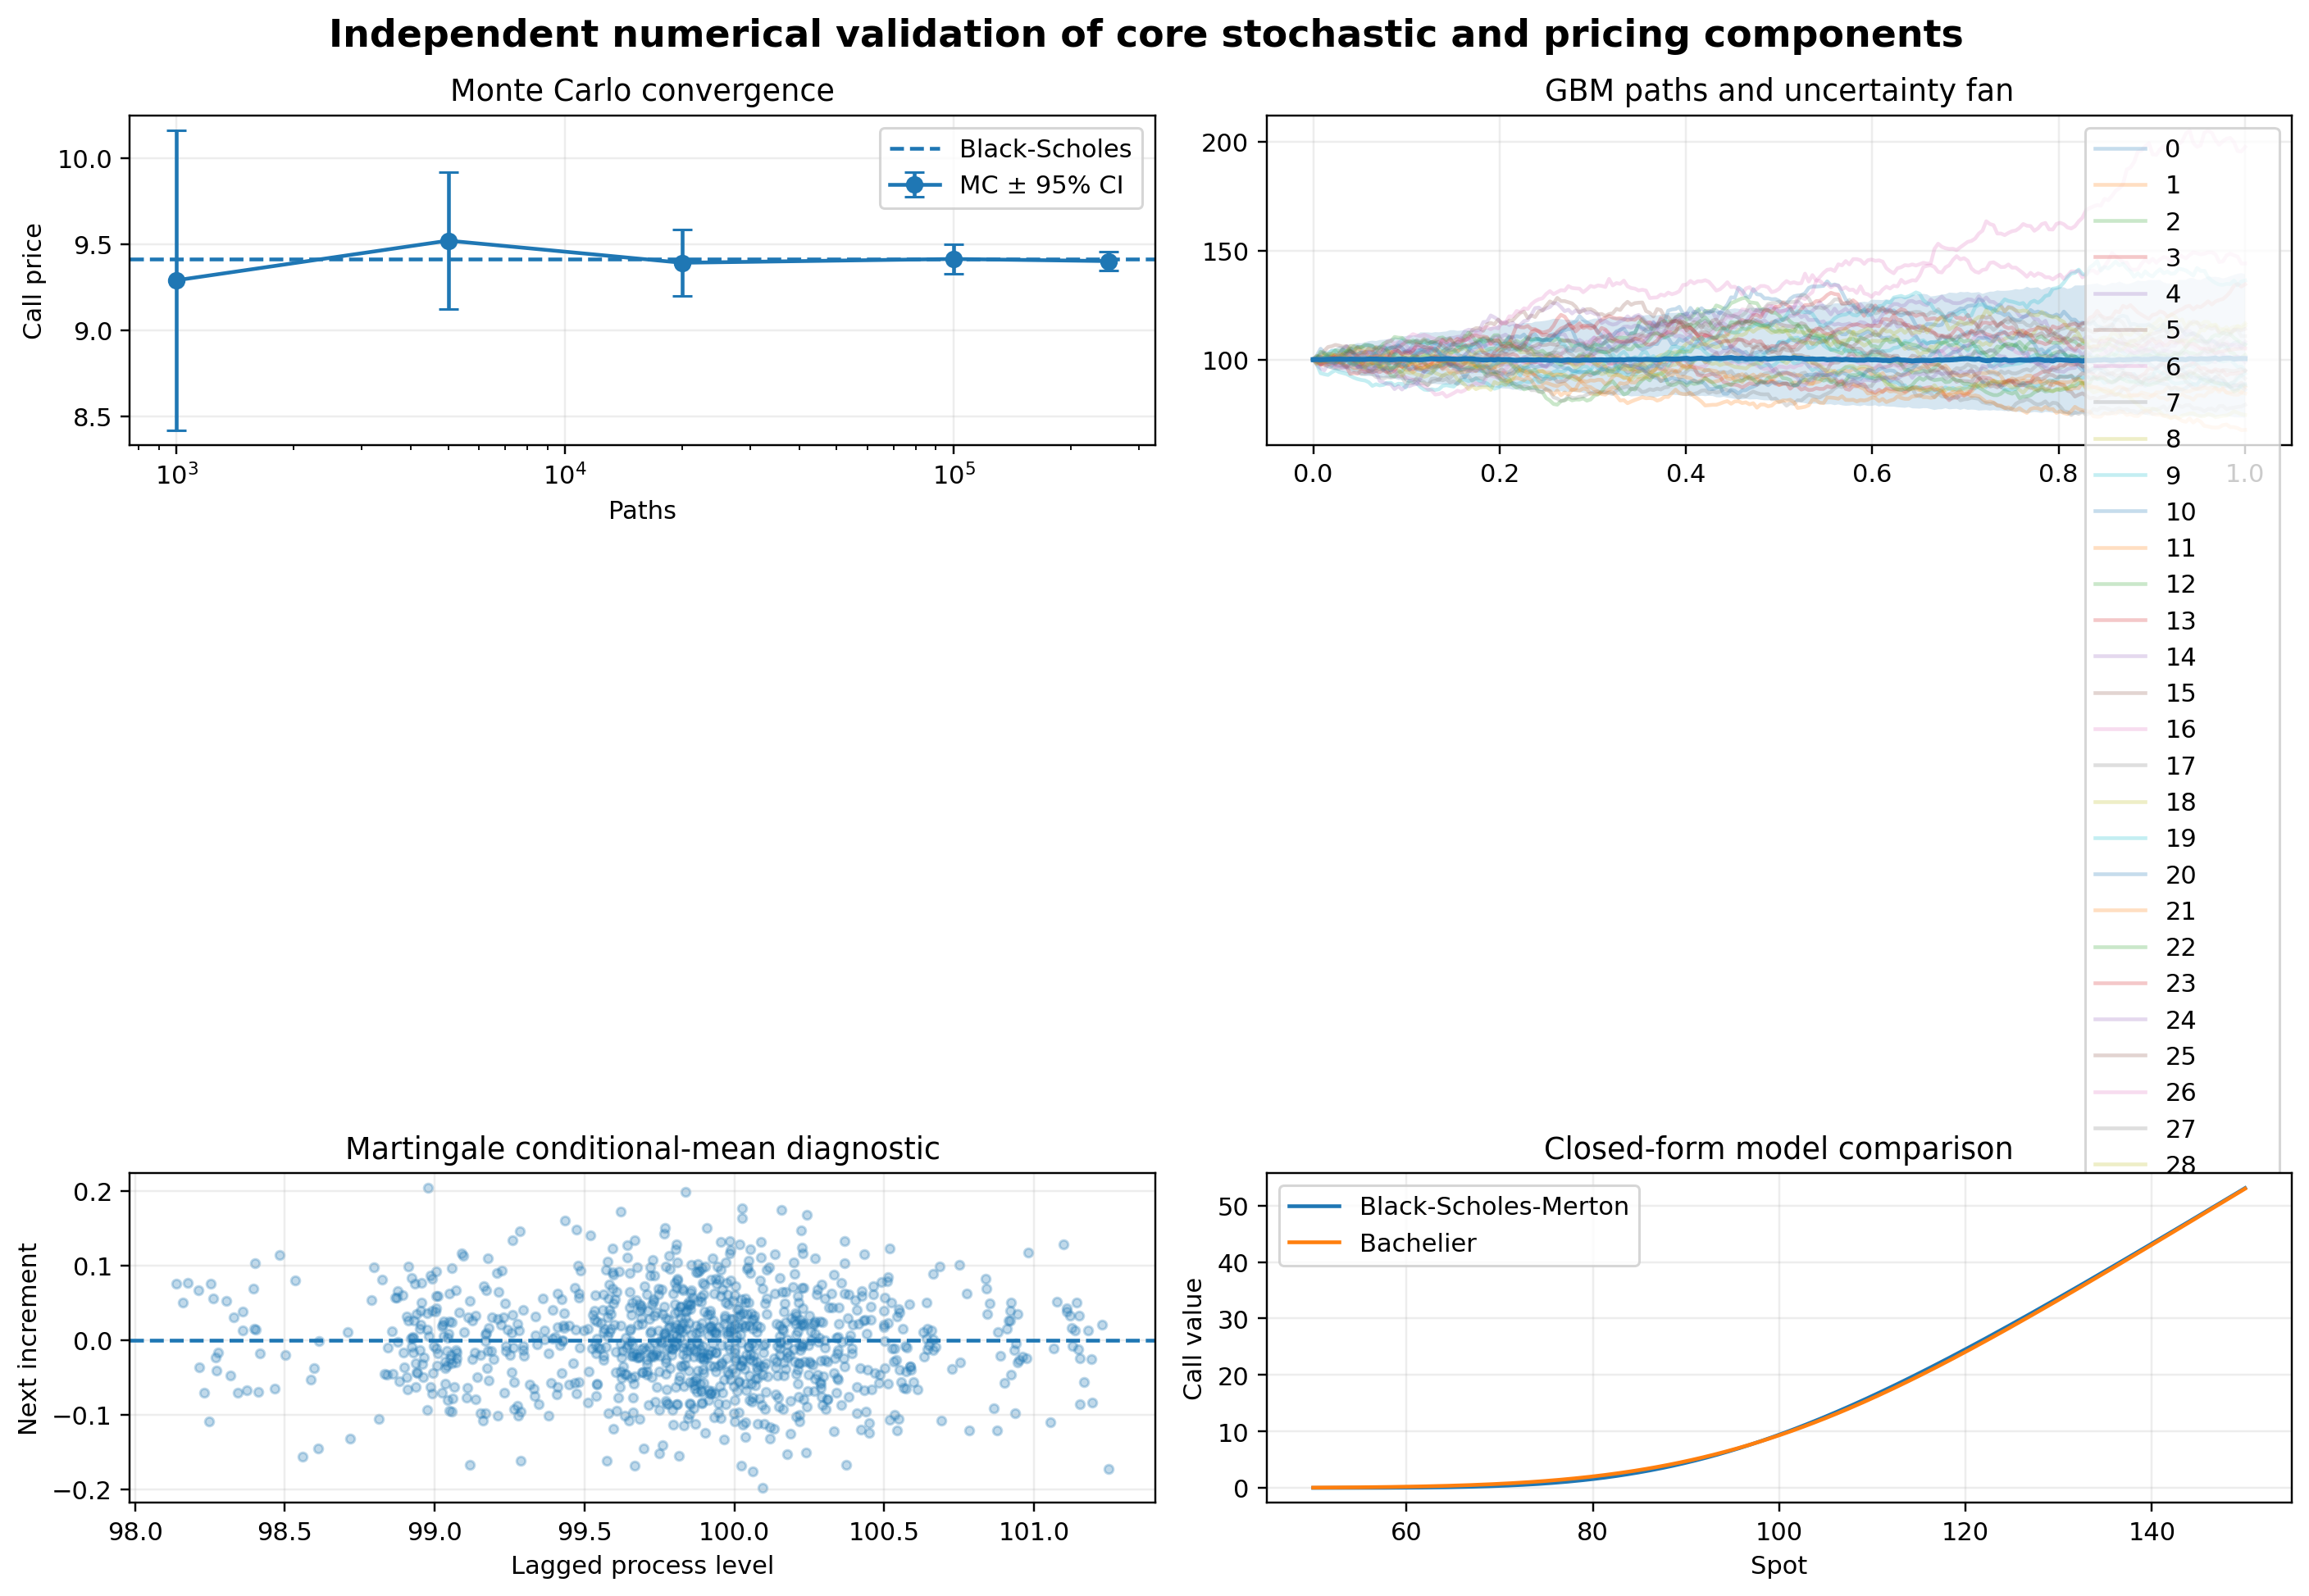
\includegraphics[width=0.96\textwidth]{figures/extended_validation_v100.png}
\caption{Numerical validation panels: Monte Carlo convergence to Black--Scholes--Merton, GBM path uncertainty, a finite-sample martingale diagnostic, and a Black--Scholes/Bachelier model comparison.}
\label{fig:extended-validation}
\end{figure}

\section{Reproducibility and Provenance}

A result object stores the validated prices, asset returns, target weights, effective weights, gross and net returns, equity, turnover, total cost, cost decomposition, specification, and metadata. A manifest records:

\begin{itemize}
  \item UTC creation timestamp;
  \item Python, operating-system, NumPy, and pandas versions;
  \item data fingerprint;
  \item specification fingerprint;
  \item combined experiment fingerprint;
  \item user-supplied metadata such as dataset version, source, or research issue.
\end{itemize}

The self-contained HTML report embeds figures as base64 data. This avoids broken relative image links when a report is moved or archived. The source repository also includes \texttt{CITATION.cff}, an MIT license, a contributor guide, a code of conduct, continuous-integration workflow, and benchmark scripts.

\section{Empirical Evaluation}

\subsection{Objectives}

The evaluation does not attempt to demonstrate a profitable trading strategy. It assesses four software properties:

\begin{enumerate}
  \item deterministic end-to-end execution;
  \item visibility of cost and timing sensitivity;
  \item ability to produce research diagnostics and figures;
  \item practical runtime scaling for vectorized experiments.
\end{enumerate}

\subsection{Synthetic market}

We use a two-state regime-switching generator with Markov transition matrix

\begin{equation}
 \Pi=
 \begin{pmatrix}
 0.97 & 0.03\\
 0.08 & 0.92
 \end{pmatrix}.
\end{equation}

State 0 has annualized drift $8\%$ and volatility $12\%$; state 1 has annualized drift $-12\%$ and volatility $32\%$. Asset shocks have pairwise correlation $0.35$. Prices are generated by exponentiating cumulative log returns. Random seeds are fixed in the benchmark script.

\subsection{Reference strategy}

The logical strategy is a moving-average crossover. For fast window $f$ and slow window $s>f$,

\begin{equation}
 z_{t,i}^{\mathrm{raw}}=
 \mathbf{1}\left\{
 \operatorname{SMA}_{f}(P_{\cdot,i})_t>
 \operatorname{SMA}_{s}(P_{\cdot,i})_t
 \right\}.
\end{equation}

Active long signals are normalized cross-sectionally to unit gross exposure. Unless otherwise stated, $f=20$, $s=100$, execution delay is one bar, and linear transaction cost is 5 basis points per unit of turnover.

\subsection{Reference result}

The reference experiment contains 1,500 business-day observations and four assets. It intentionally produces a negative result, avoiding the implication that the software example has been selected for profitability.

\begin{table}[H]
\centering
\caption{Selected reference metrics.}
\begin{tabular}{lr}
\toprule
Metric & Value \\
\midrule
Total return & -21.4705\% \\
CAGR & -3.9792\% \\
Annual volatility & 14.9722\% \\
Sharpe ratio & -0.1963 \\
Sortino ratio & -0.2710 \\
Maximum drawdown & -34.2904\% \\
Expected Shortfall 95\% & 2.4404\% \\
Average turnover per bar & 3.9778\% \\
Annualized turnover & 10.0240 \\
\bottomrule
\end{tabular}
\end{table}

\begin{figure}[H]
\centering
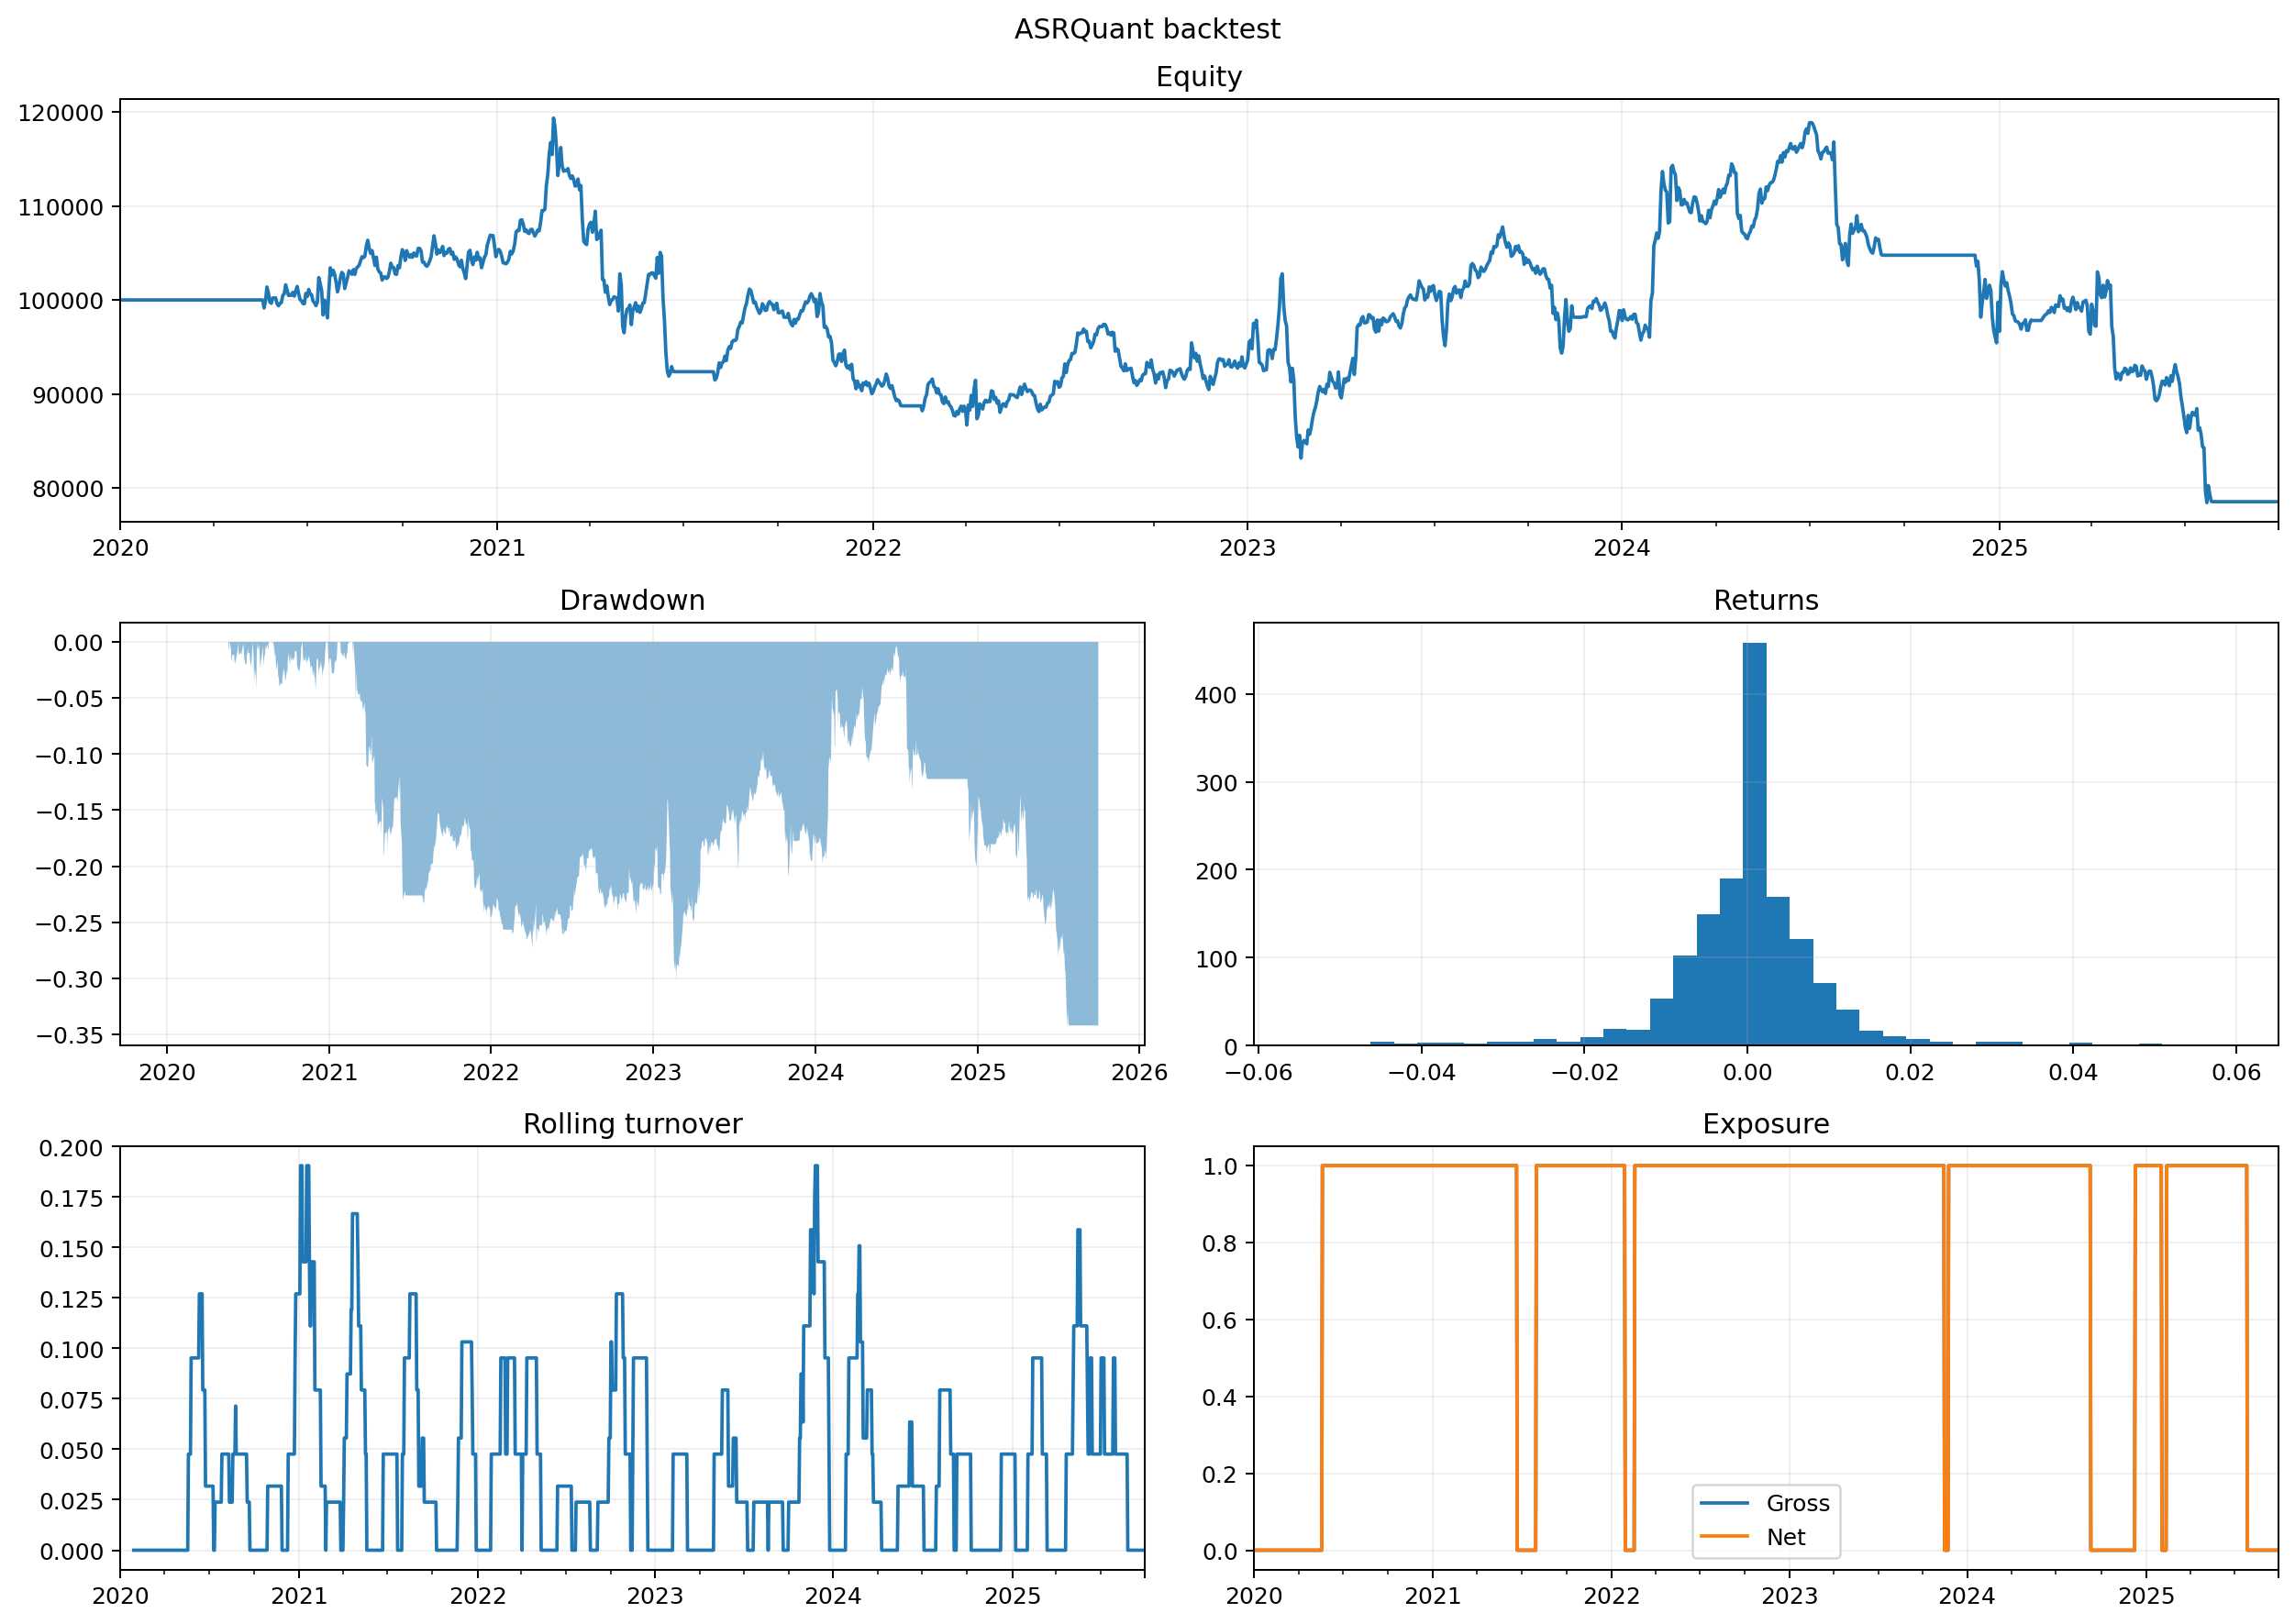
\includegraphics[width=\textwidth]{figures/dashboard.png}
\caption{Reference dashboard combining equity, drawdown, return distribution, turnover, and exposure.}
\label{fig:dashboard}
\end{figure}

\subsection{Implementation audit: stable negative conclusion}

The first audit combines three delays $\{0,1,2\}$, four linear cost levels $\{0,5,10,25\}$ basis points, and two rebalancing conventions (every bar and month-end), for 24 contracts. Total return ranges from -30.34\% to -9.16\%. The return sensitivity is 21.18 percentage points, but every contract remains negative, so the sign-based conclusion stability index equals one. This example distinguishes metric instability from conclusion instability.

\begin{figure}[H]
\centering
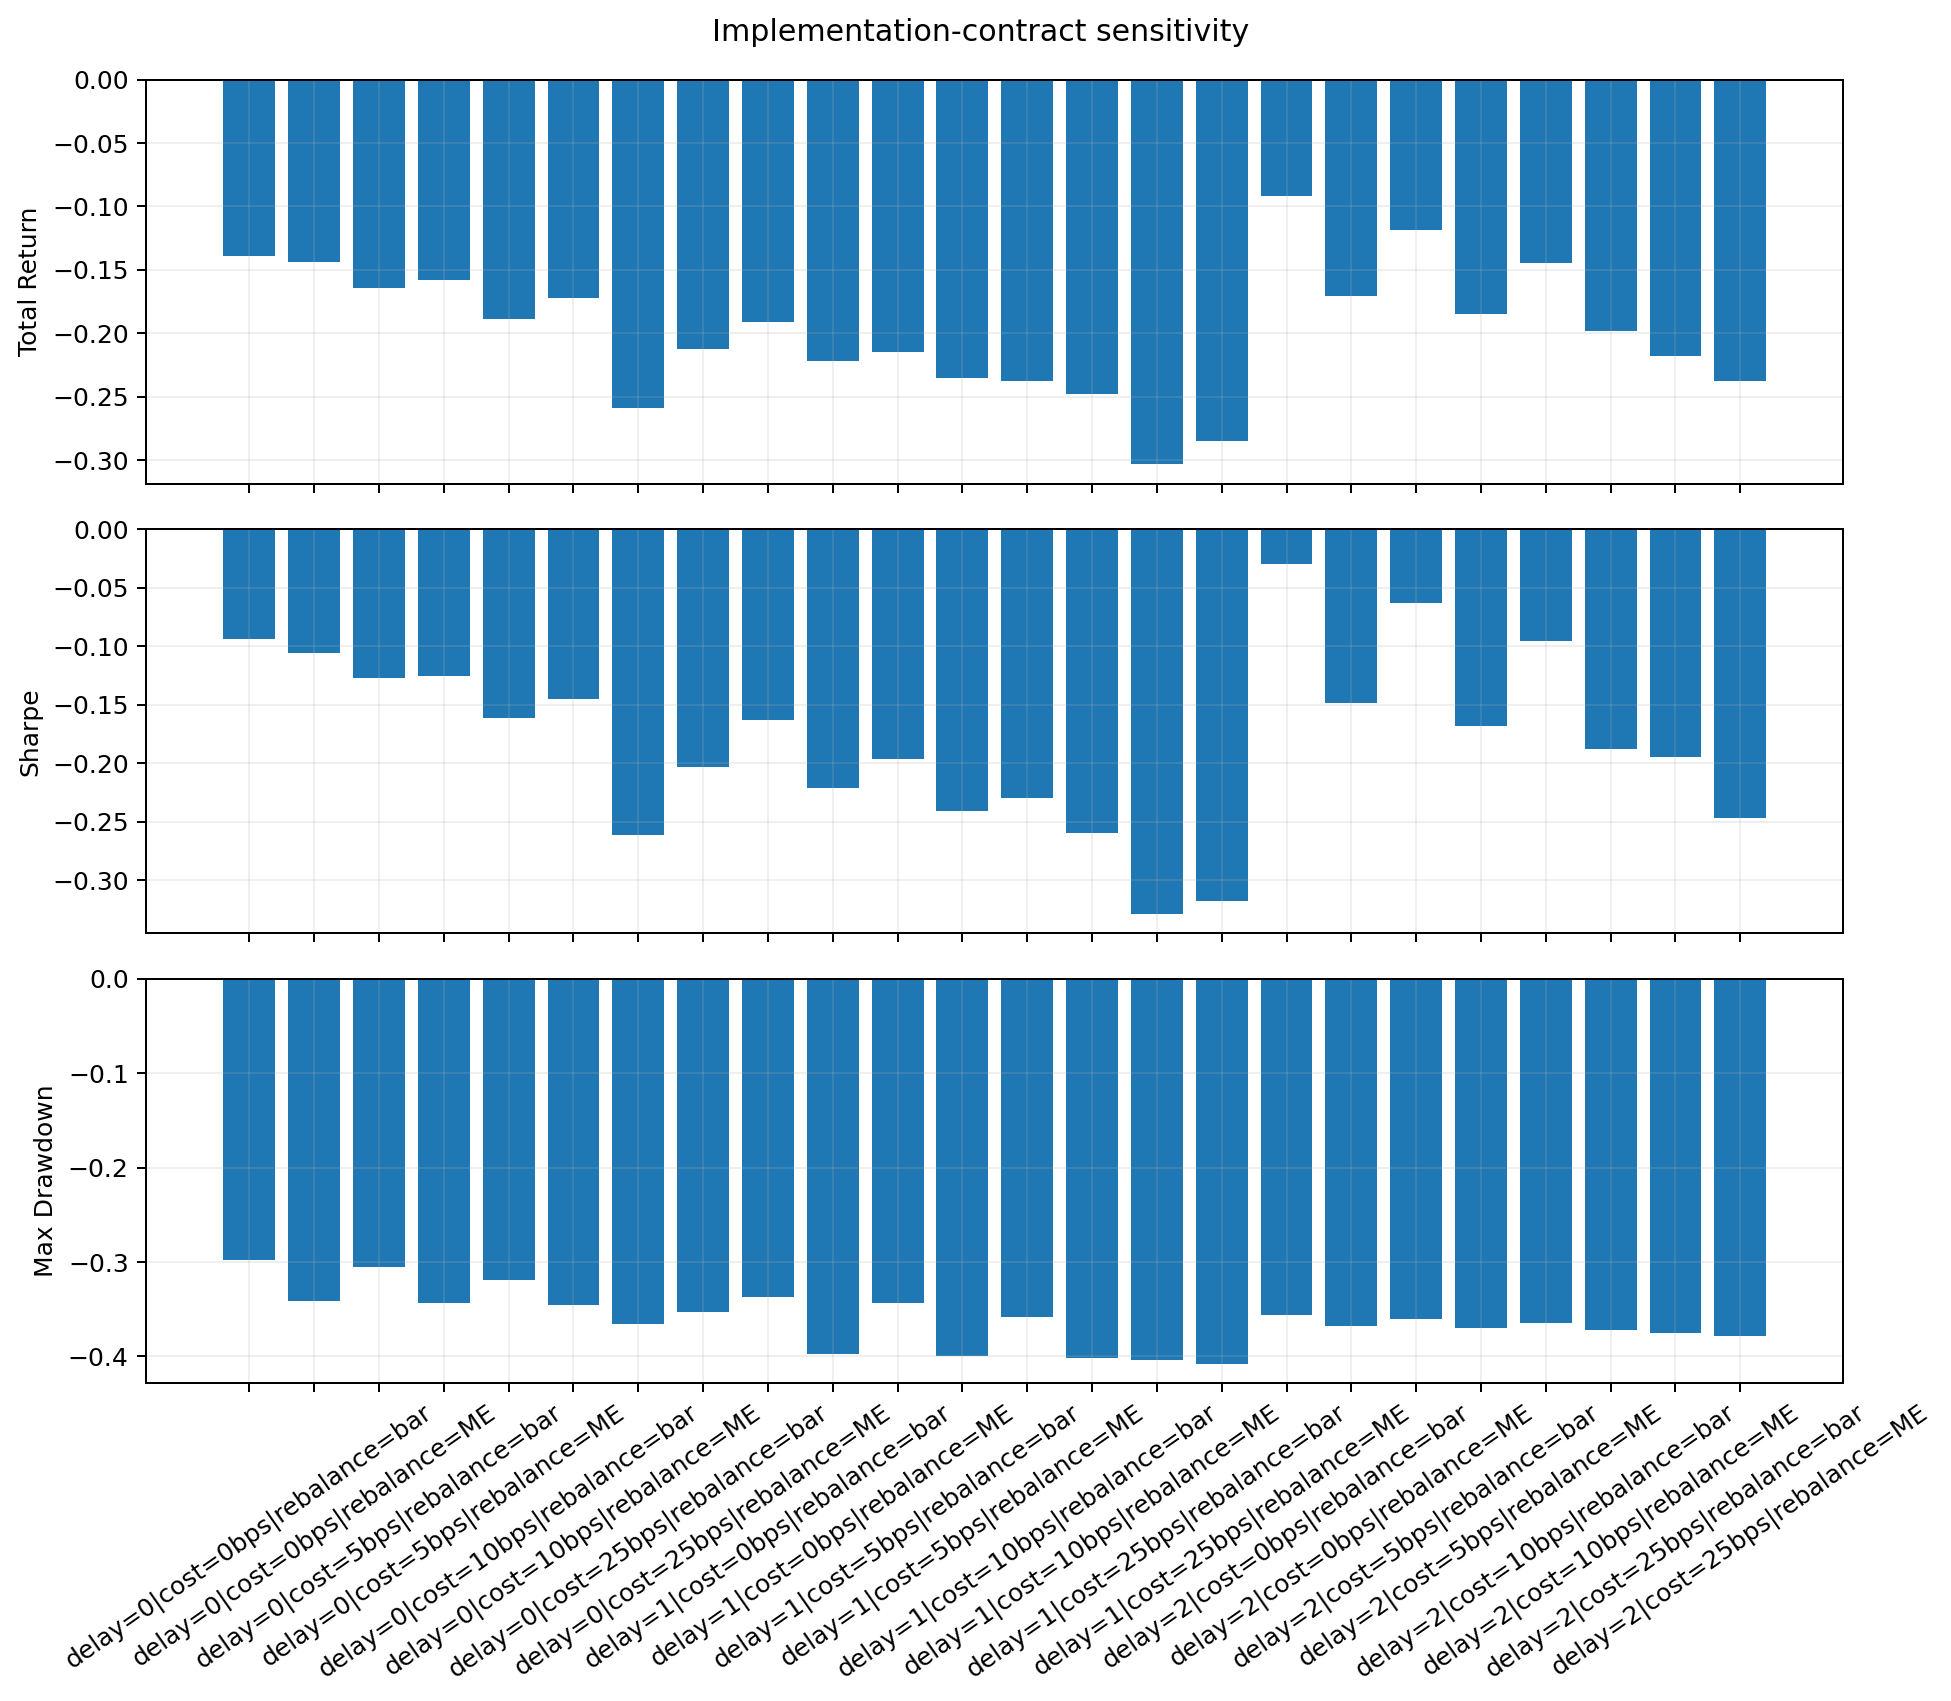
\includegraphics[width=\textwidth]{figures/implementation_audit.png}
\caption{Selected metrics under 24 implementation contracts. The sign is stable, but magnitude is not.}
\label{fig:auditstable}
\end{figure}

\subsection{Implementation audit: fragile conclusion}

A shorter 500-bar, three-asset experiment with fast window 10 and slow window 40 illustrates a fragile edge. Table~\ref{tab:fragile} reports all six contracts.

\begin{table}[H]
\centering
\caption{Fragile strategy under execution and cost alternatives.}
\label{tab:fragile}
\begin{tabular}{rrrrr}
\toprule
Delay & Cost (bps) & Total return & Sharpe & Max drawdown \\
\midrule
0 & 0 & 12.5975\% & 0.4777 & -10.6600\% \\
0 & 5 & 10.1847\% & 0.4040 & -10.8532\% \\
0 & 10 & 7.8224\% & 0.3301 & -11.2408\% \\
1 & 0 & 1.9718\% & 0.1405 & -13.3180\% \\
1 & 5 & -0.2094\% & 0.0684 & -13.6062\% \\
1 & 10 & -2.3450\% & -0.0039 & -13.8936\% \\
\bottomrule
\end{tabular}
\end{table}

The implementation uncertainty interval for total return is $[-2.3450\%,12.5975\%]$, the return sensitivity is 14.94 percentage points, and the sign-based conclusion stability index is $1/3$. A researcher reporting only the same-bar, zero-cost result would communicate a materially different conclusion from a researcher using the package default plus modest costs.

\begin{figure}[H]
\centering
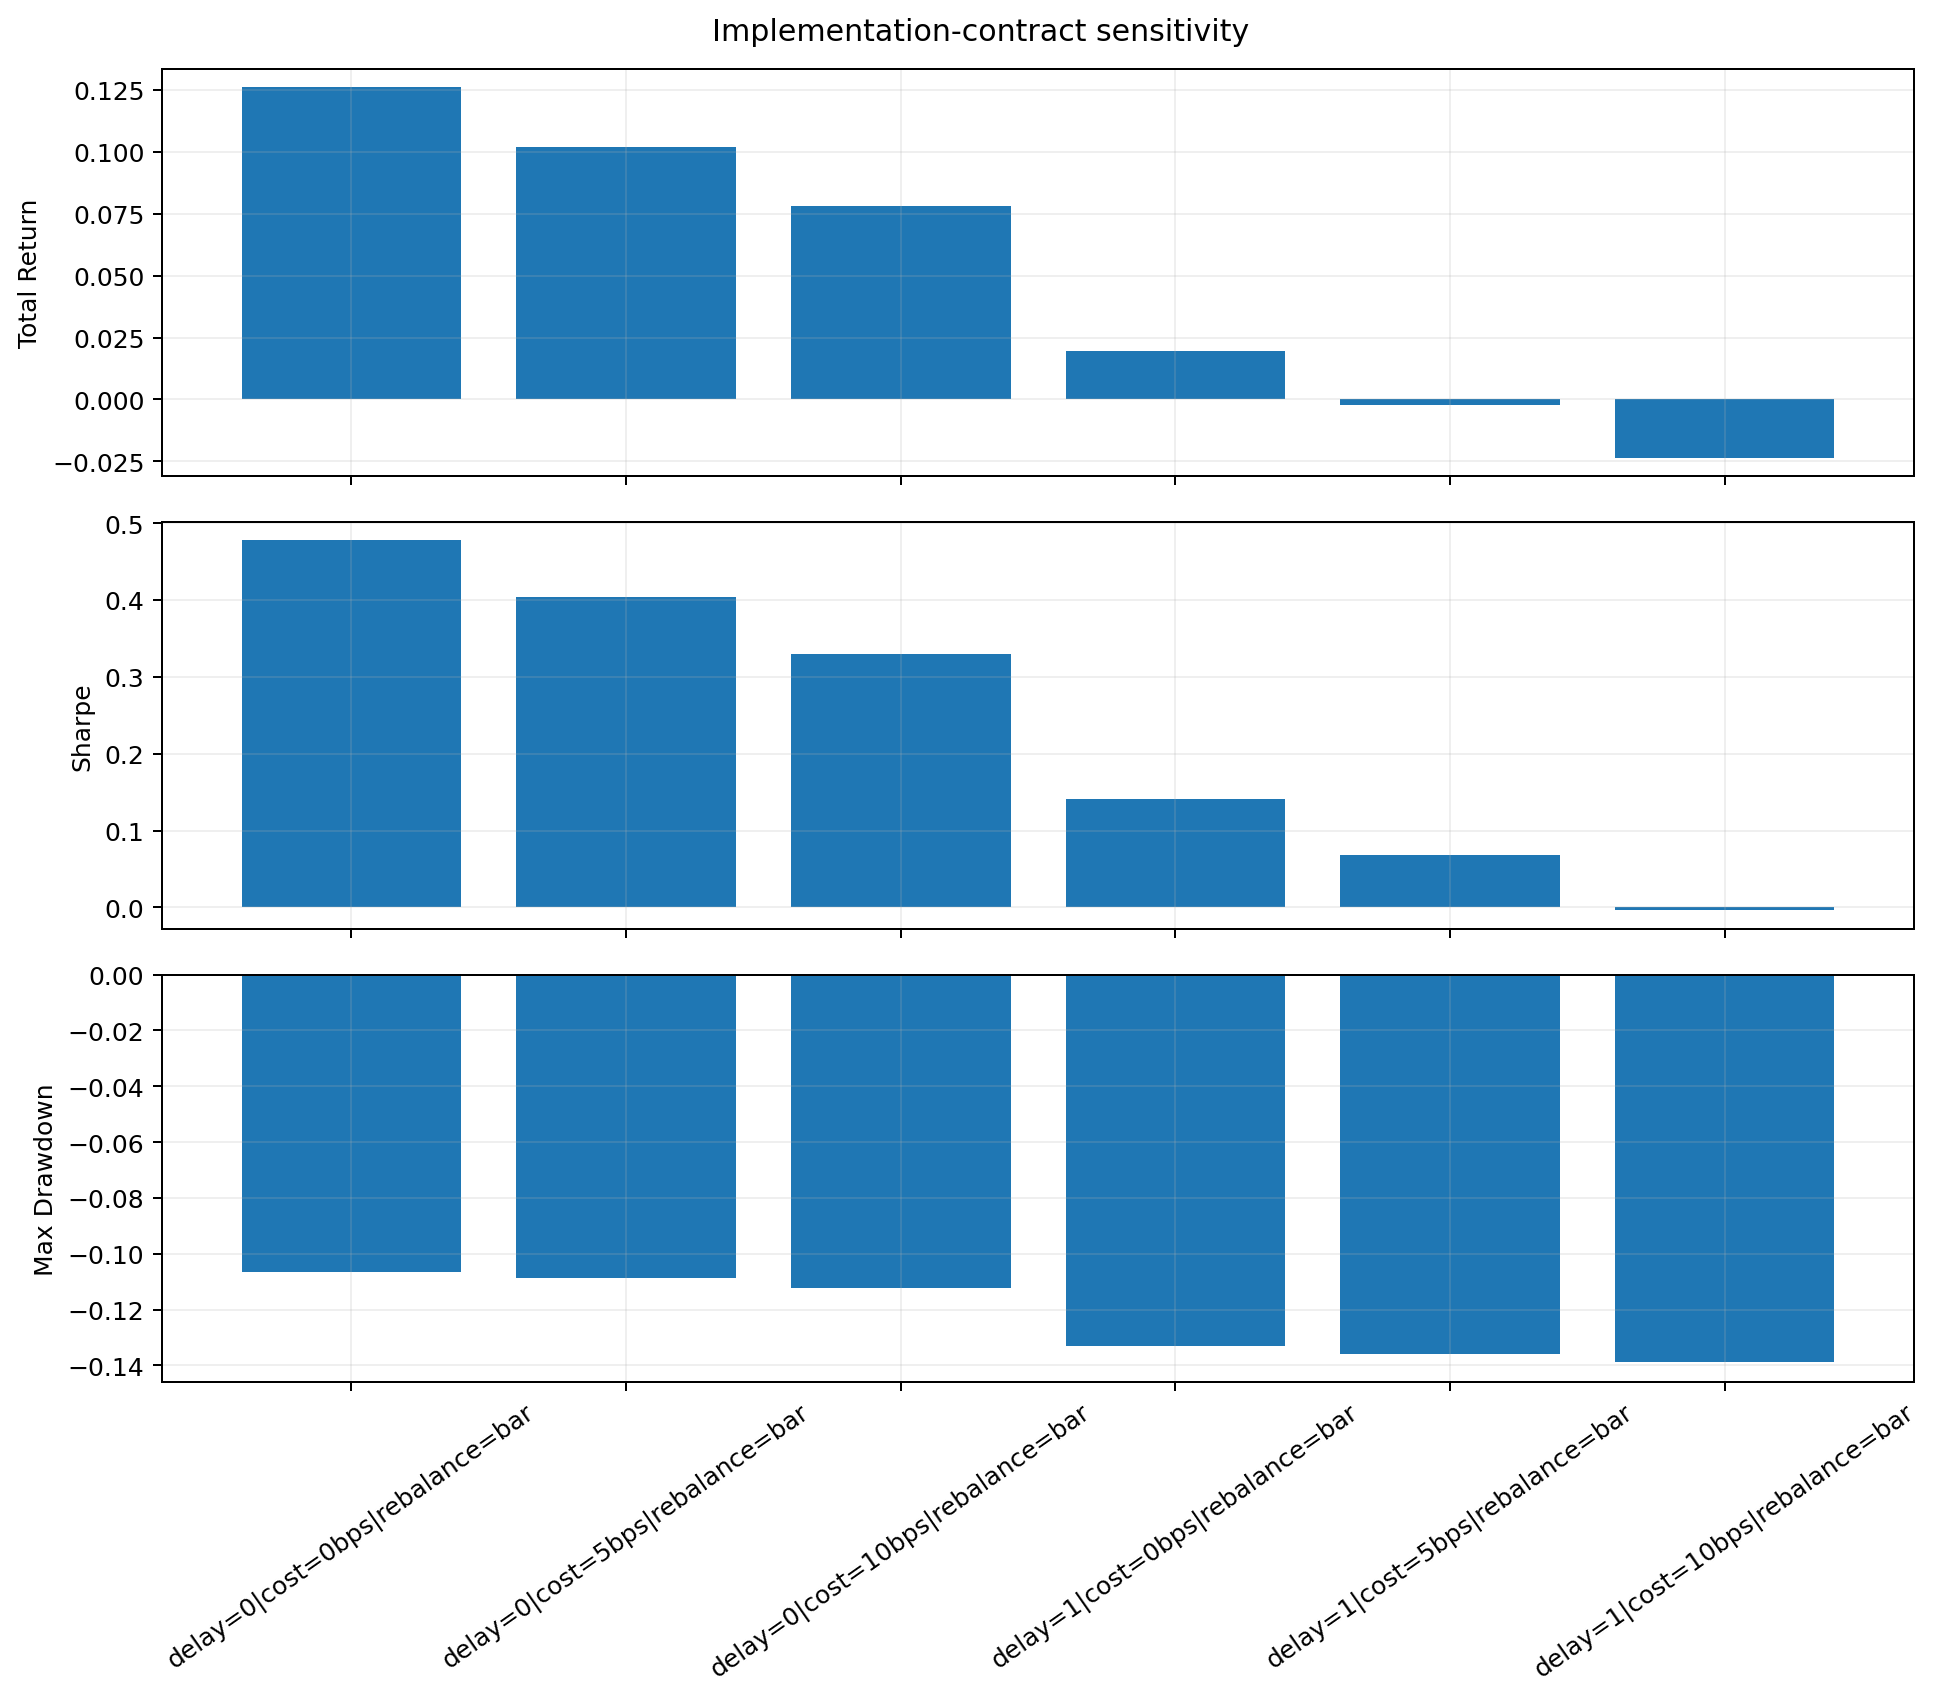
\includegraphics[width=\textwidth]{figures/fragile_implementation_audit.png}
\caption{Fragile strategy audit. The sign changes when a one-bar delay and realistic costs are introduced.}
\label{fig:auditfragile}
\end{figure}

\subsection{Parameter landscapes and multidimensional animation}

A geometric response surface displays two parameters. Let $g(\theta)$ denote any experiment returning an object and let $m$ be a scalar metric selector. For displayed axes $x_i$ and $y_j$, fixed parameters $c$, and an animation-frame configuration $\phi_k$, \pkg evaluates

\begin{equation}
Z_{kij}=m\!\left(g(x_i,y_j,\phi_k,c)\right).
\end{equation}

The frame configuration may itself contain several parameters. If $\Phi_1,\ldots,\Phi_q$ are the selected animation dimensions, the ordered frame table is the Cartesian product

\begin{equation}
\mathcal{F}=\Phi_1\times\cdots\times\Phi_q.
\end{equation}

This construction does not pretend that a literal surface can have more than two geometric axes. It represents higher-dimensional experiments as a reproducible sequence of two-dimensional slices. Frame values may be numeric, Boolean, or categorical, allowing examples such as risk aversion and cost on the axes while hedge frequency, volatility regime, model family, and random seed determine the animation frames. The metric selector may be a mapping key, dotted object path such as \texttt{metrics.Sharpe}, or an arbitrary reduction callback.

Parameter sweeps can be visualized as heatmaps, contours, three-dimensional surfaces, or interactive HTML animations with a parameter slider. GIF and MP4 exports are also supported, with stable global color and vertical scales to avoid visual changes caused only by automatic rescaling. Figure~\ref{fig:surface} shows Sharpe ratios across fast and slow moving-average windows under a fixed execution contract. Figure~\ref{fig:multisurface} illustrates four slices from a surface family in which two additional hedging parameters define the frames.

\begin{figure}[H]
\centering
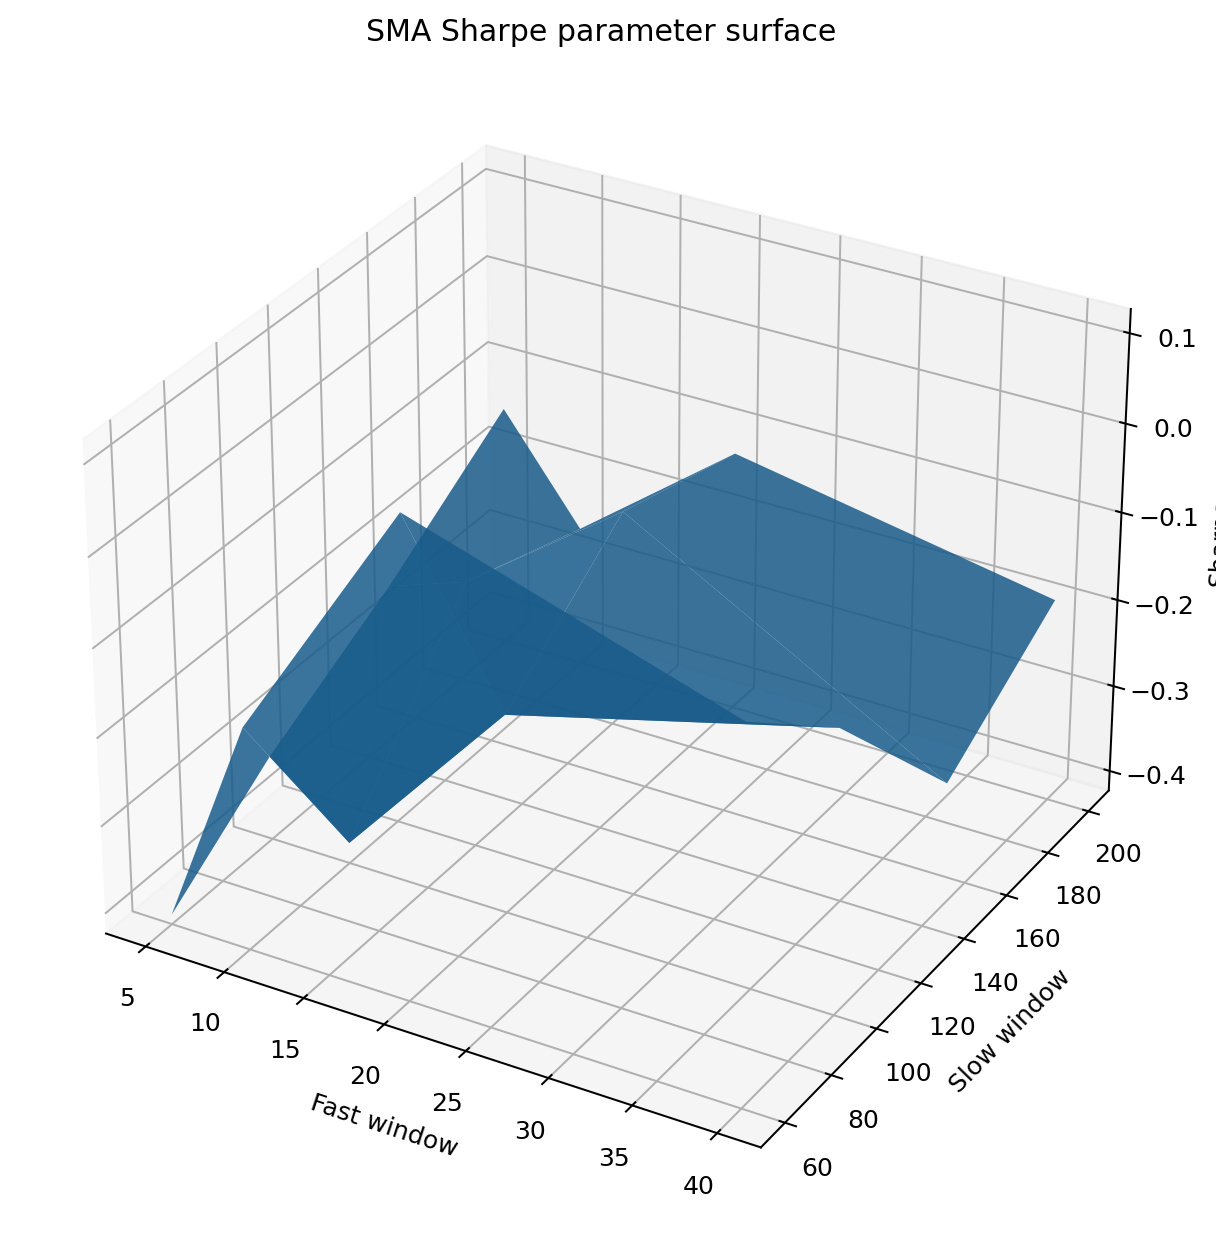
\includegraphics[width=0.82\textwidth]{figures/parameter_surface.png}
\caption{Sharpe-ratio parameter surface for moving-average windows.}
\label{fig:surface}
\end{figure}

\begin{figure}[H]
\centering
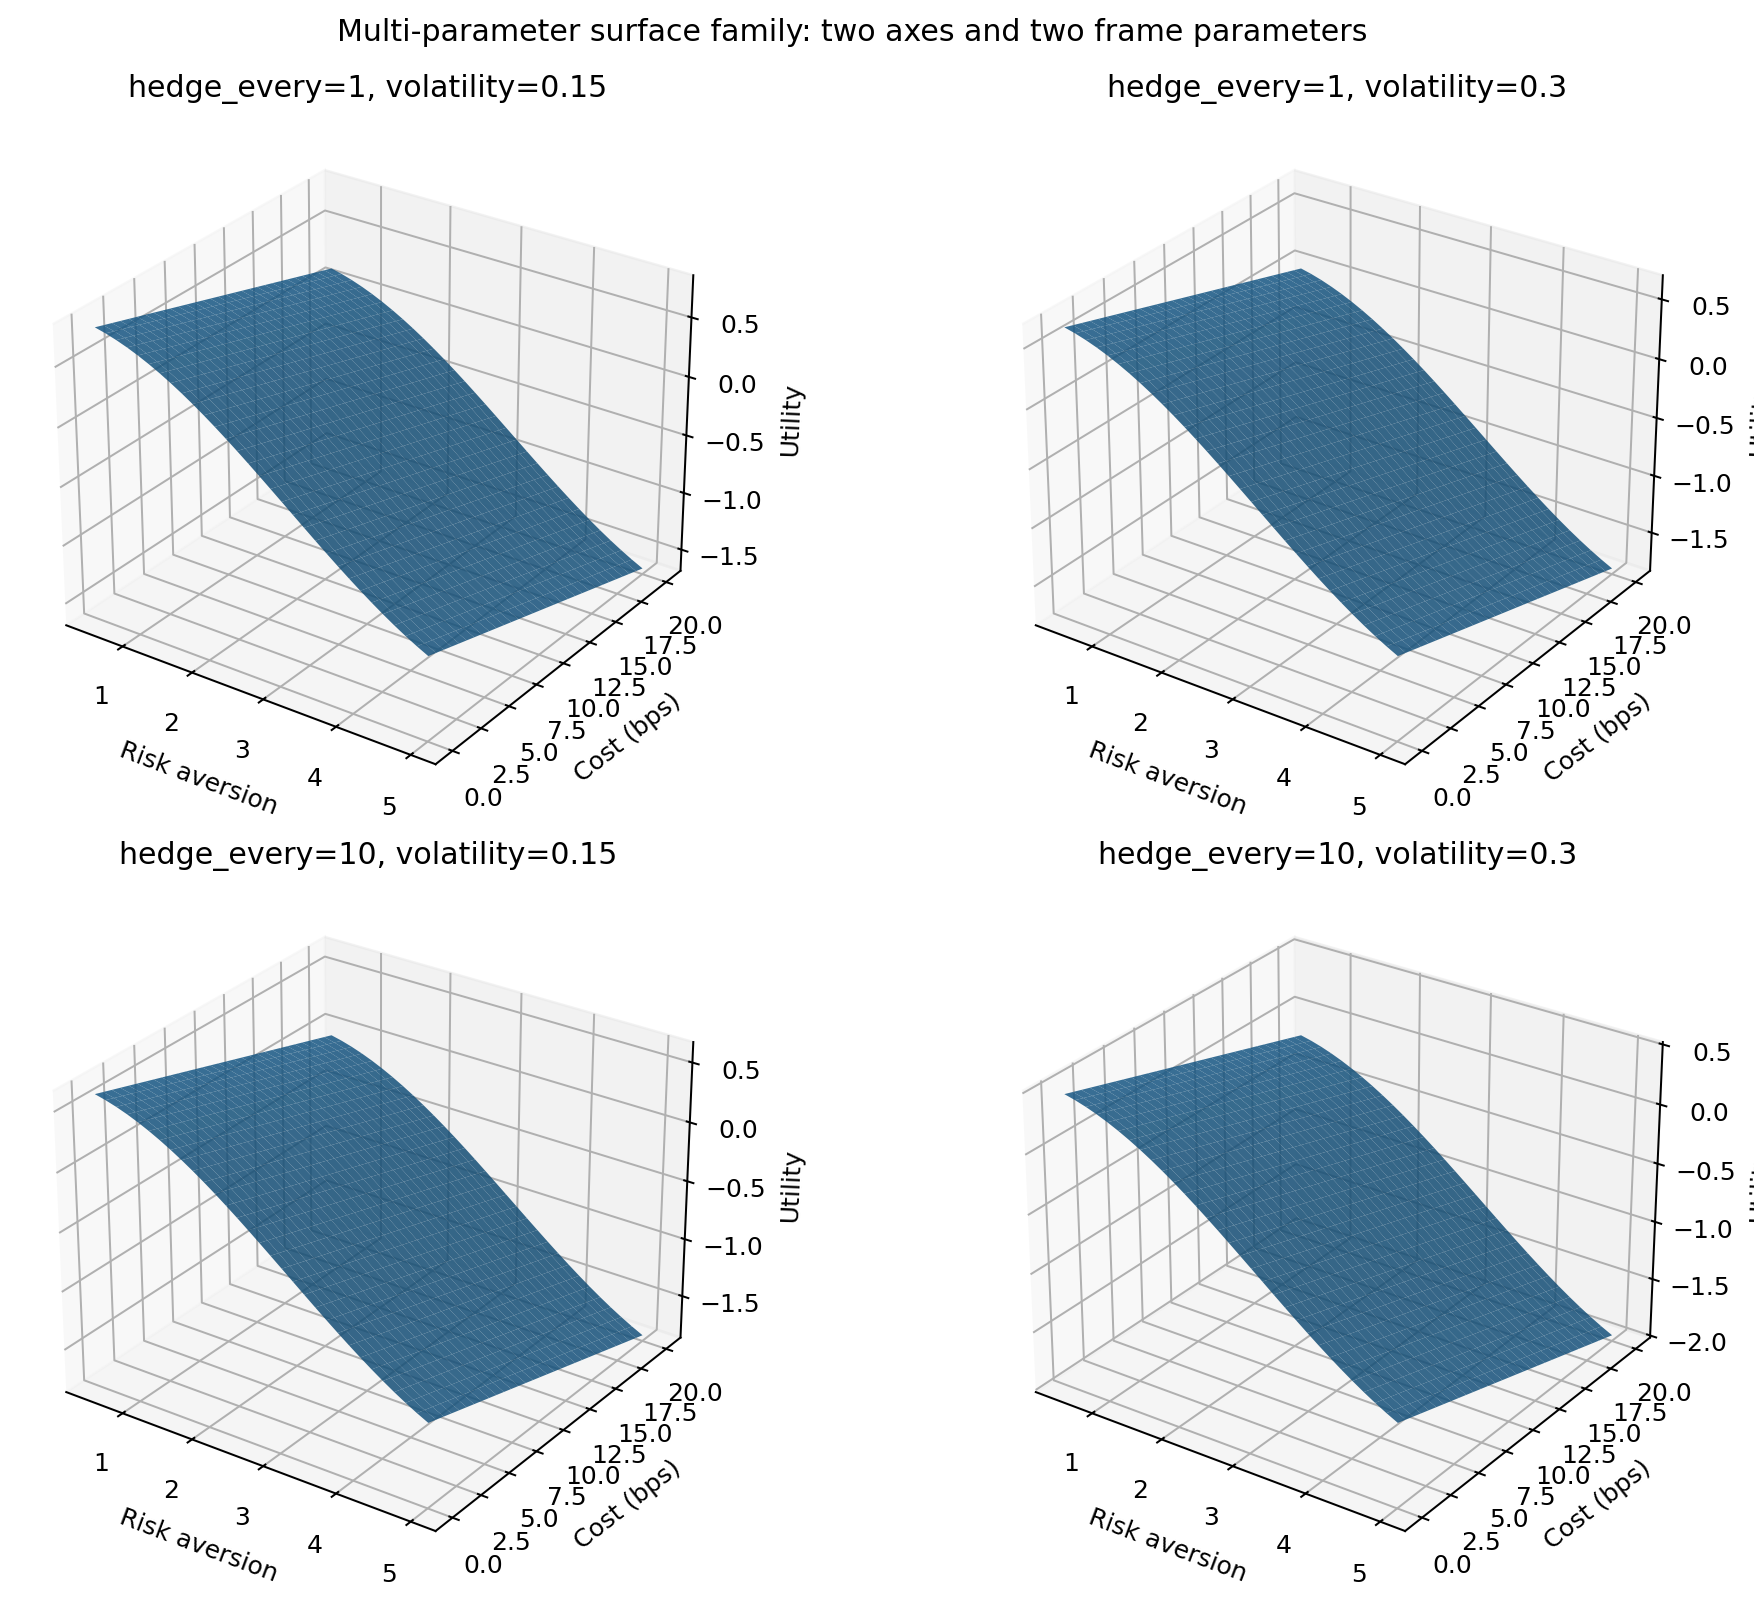
\includegraphics[width=0.96\textwidth]{figures/multidimensional_surface_v100.png}
\caption{A multidimensional parameter experiment represented by two surface axes and a Cartesian frame table over hedge frequency and volatility.}
\label{fig:multisurface}
\end{figure}

A surface does not validate a strategy. Evaluating many configurations increases selection risk, and visually smooth regions may reflect interpolation, common random numbers, or model structure rather than genuine economic robustness. The package therefore records evaluation counts, fixed parameters, frame parameters, failures, and best-point extraction, while leaving out-of-sample design and multiple-testing control to the research protocol.

\subsection{Runtime scaling}

Runtime was measured as the median of five runs after data construction on the benchmark environment. The table reports end-to-end strategy construction and backtesting. Results are environment-specific and should not be interpreted as universal performance guarantees.

\begin{table}[H]
\centering
\caption{Vectorized runtime scaling.}
\begin{tabular}{rrrr}
\toprule
Bars & Assets & Data cells & Median seconds \\
\midrule
1,000 & 1 & 1,000 & 0.0065 \\
1,000 & 10 & 10,000 & 0.0093 \\
5,000 & 10 & 50,000 & 0.0136 \\
5,000 & 50 & 250,000 & 0.0361 \\
20,000 & 50 & 1,000,000 & 0.1145 \\
\bottomrule
\end{tabular}
\end{table}

The scaling is consistent with array-oriented operations over the price and weight panels. Memory, rather than arithmetic, will become the main limitation for very large grids or high-frequency datasets.

\subsection{Independent numerical model validation}

For $S_0=K=100$, $T=1$, $r=3\%$, and $\sigma=20\%$, the analytic BSM call value is $9.413403$. Table~\ref{tab:numerical} compares independent numerical engines.

\begin{table}[H]
\centering
\caption{Independent pricing checks against the analytic BSM value.}
\label{tab:numerical}
\begin{tabular}{lrrr}
\toprule
Method & Resolution & Estimate & Absolute error \\
\midrule
Monte Carlo, antithetic & 1,000 paths & 9.289937 & 0.123466 \\
Monte Carlo, antithetic & 20,000 paths & 9.391629 & 0.021774 \\
Monte Carlo, antithetic & 100,000 paths & 9.413542 & 0.000139 \\
CRR binomial & 100 steps & 9.393596 & 0.019808 \\
CRR binomial & 1,000 steps & 9.411420 & 0.001983 \\
\bottomrule
\end{tabular}
\end{table}

The 100,000-path Monte Carlo 95\% interval is $[9.326114,9.500970]$, containing the analytic value. Error need not decline monotonically for one random sequence, but the standard error scales approximately as $N^{-1/2}$. The tree error decreases as the time grid is refined.

A zero-drift arithmetic Brownian sample with 1,008 increments produced p-values $0.4493$ for zero mean, $0.3314$ for lagged-level predictability, and $0.7927$ for Ljung--Box autocorrelation. These are non-rejections in one controlled sample, not evidence that a market price series is a martingale. In a separate 1,500-observation factor simulation with true coefficients $(\alpha,\beta_M,\beta_V)=(0.0002,1.25,-0.40)$, HAC estimates were $(0.000276,1.25523,-0.39490)$ and all true values lay within the reported 95\% intervals. These checks test formula wiring, alignment, and numerical convergence rather than economic usefulness.

\section{Verification and Testing}

The stable release contains 154 automated tests, including an 18-test paper-contract suite that executes the public workflows and capability claims used in this manuscript. The full suite spans:

\begin{itemize}
  \item specification fingerprints and validation;
  \item missing-data policies and data fingerprints;
  \item OHLC consistency;
  \item buy-and-hold return identity;
  \item cost monotonicity and execution-delay sensitivity;
  \item leverage and weight constraints;
  \item one-import and five-line API workflows, local-file ingestion, provider-response normalization, CLI commands, and HTML report generation;
  \item an 18-test paper-contract suite covering the appendix workflows, PDF-to-hypothesis ingestion, all seven core process families, derivatives, fixed income, broker order states and partial fills, surface export, and formula-to-polynomial modelling;
  \item performance, benchmark, drawdown, volatility, and tail-risk metrics;
  \item implementation-audit grids, trade ledgers, strategy comparisons, and parameter sweeps;
  \item static, single-frame, and multi-parameter surface evaluation, categorical frame tables, dotted metric extraction, parallel execution, error recovery, Plotly HTML export, and multidimensional backtest animations;
  \item walk-forward, gap-aware, and purged temporal splits;
  \item ABM, GBM, Heston, and jump-process simulation invariants;
  \item Monte Carlo pricing against Black--Scholes--Merton and CRR convergence;
  \item Bachelier, Black--76, put--call parity, implied-volatility recovery, and option dispatch;
  \item martingale diagnostics under controlled driftless processes;
  \item portfolio optimizer constraints, covariance estimators, HRP, Black--Litterman, and risk parity;
  \item OLS/HAC coefficient recovery, robust and regularized regressions, bootstrap, stationarity, FDR, and walk-forward ML;
  \item bond, yield, duration, convexity, and volatility-estimator checks;
  \item smoke tests for market, performance, risk, stochastic, portfolio, regression, derivative, ML, and microstructure figures.
\end{itemize}

All tests pass in the artifact environment used to produce this paper. Visual tests check successful figure construction rather than pixel-perfect rendering, because minor renderer differences should not fail scientific calculations.

\section{Comparison with Existing Workflows}

\begin{table}[H]
\centering
\caption{Qualitative design comparison. This table describes primary emphasis, not every optional feature of each project.}
\begin{tabularx}{\textwidth}{lccccX}
\toprule
Project & Backtest & Tear sheet & Broad viz & Contract audit & Primary emphasis \\
\midrule
backtesting.py & Yes & Partial & Partial & No & Concise event-oriented strategy testing. \\
vectorbt & Yes & Yes & Strong & Partial/custom & High-performance vectorized research. \\
pyfolio & No & Yes & Performance & No & Portfolio performance and risk analytics. \\
QuantStats & No & Yes & Performance & No & Return-stream profiling and reports. \\
\pkg & Yes & Yes & Cross-domain & Yes & Explicit semantics plus integrated research diagnostics. \\
\bottomrule
\end{tabularx}
\end{table}

The comparison is not intended to rank mature specialist projects against ASRQuant 1.0.0; it compares primary workflow emphasis only. \pkg can interoperate with them: external engines can supply returns or weights, and future adapters can compare their results under a common contract.

\section{Limitations}

\subsection{Execution realism}

The vectorized reference backtest is weight-based and bar-based. The separate deterministic paper broker supports order states, market/limit/stop/stop-limit primitives and configurable partial fills, but neither component models exchange queue priority, venue-specific fee schedules, latency, full intrabar paths, market halts, auction mechanics, or stochastic queue fills. Researchers working at high frequency should use a specialist event-driven or exchange simulator and can still use \pkg for analytics, audit and visualization.

\subsection{Corporate actions and point-in-time data}

The package validates numerical panels but does not supply a corporate-action database or point-in-time fundamental data. Split adjustment, dividends, delistings, survivorship, restatements, and publication lags must be handled upstream and documented in the manifest.

\subsection{Transaction-cost calibration}

Basis-point costs and power-law impact are simplified models. Calibrated execution costs should depend on spread, volatility, volume, participation, order type, and market state. A visually attractive cost plot cannot compensate for weak calibration.

\subsection{Statistical inference}

The included DSR is an approximation and depends on the declared number of trials. The framework cannot infer unrecorded experiments. Block-bootstrap validity depends on stationarity and block-length choices. Regression p-values are not causal evidence.

\subsection{Visualization risk}

Plots can encourage narrative overfitting. Parameter surfaces, animations, regime colors, and three-dimensional figures are descriptive tools. A large Cartesian grid increases selection opportunities and computational cost. Surfaces should be accompanied by pre-specified hypotheses, genuine out-of-sample evaluation, multiple-testing control where appropriate, and uncertainty analysis. Stable frame scales prevent one visual artifact but do not establish robustness.

\subsection{Optimization instability}

Mean--variance solutions can be highly sensitive to estimated means and covariances. The package includes shrinkage estimators, HRP, risk parity, maximum diversification, and Black--Litterman, but these methods do not remove estimation risk. Distributionally robust optimization, explicit posterior-uncertainty propagation, taxes, integer lots, and transaction-aware multi-period optimization remain outside the current release.

\subsection{Package maturity}

ASRQuant 1.0.0 is the first stable public-API release described by this manuscript. Here, ``stable'' refers to the package interface, reproducible research contracts, tested numerical pathways, and distribution format; it does not mean that every research result is economically valid or that any installation is authorized for live capital. Future incompatible API changes follow semantic-versioning rules, while live deployment remains a separate, fail-closed operational decision.

\section{Ethical and Practical Use}

The package is not financial advice and does not predict future returns. A backtest may be technically correct and economically irrelevant. Researchers should disclose data sources, availability timestamps, costs, rejected specifications, and all material implementation decisions. Users should avoid presenting synthetic or in-sample results as evidence of deployable profitability. Sensitive or proprietary data should not be embedded in public HTML reports or manifests.

\section{Roadmap}

The implemented scope is intentionally broad, but not equivalent to a production trading platform or a complete replacement for specialist libraries. Priority extensions are:

\begin{enumerate}
  \item an event-driven engine with orders, partial fills, limit logic, corporate actions, borrow recalls, and venue calendars;
  \item authenticated WebSocket feeds, persistent storage, and broker adapters separated from the research package by strict safety boundaries;
  \item point-in-time fundamentals, vintage macro data, security-master identifiers, delistings, and survivorship controls;
  \item local-volatility, SABR, Hull--White, affine term-structure, credit, exotic, and adjoint-differentiation engines;
  \item calibrated volume, spread, square-root impact, capacity, and queue-position models;
  \item nested and combinatorial purged validation, Probability of Backtest Overfitting, White Reality Check, SPA, and complete experiment ledgers;
  \item robust and distributionally robust optimization, turnover constraints, taxes, integer lots, and multi-period allocation;
  \item distributed, JIT, GPU, adaptive sampling, surrogate modelling, and out-of-core execution for very large parameter grids;
  \item typed plugin protocols, stable serialized schemas, visual regression tests, and a versioned documentation site.
\end{enumerate}

\section{Conclusion}

\pkg demonstrates that ease of use and scientific rigor need not be opposites. A small public API can unify local and remote data, stochastic simulation, martingale diagnostics, closed-form and numerical pricing, econometrics, machine learning, portfolio construction, multidimensional parameter exploration, visualization, and backtesting, provided that the underlying assumptions remain explicit. The central design choice is therefore not maximal automation; it is auditable automation. Simulations retain seeds and parameters, Monte Carlo prices retain uncertainty, regressions retain robust diagnostics, ML retains chronological folds, and backtests retain the execution contract, costs, trade ledger, and implementation sensitivity.

The numerical checks confirm internal consistency across independent engines, but they do not validate any trading hypothesis. Likewise, access to intraday or polled data does not make the package a production execution system. The appropriate use of \pkg is to shorten reproducible quantitative research while making it harder to forget the choices that determine the result.

\appendix
\section{Five-Line Workflows}

Every snippet in this appendix is covered by the dedicated paper-contract test group. External-provider examples replace the network call with a deterministic provider stub in continuous integration, while exercising the same public API.

\subsection{CSV to audited backtest}

\begin{lstlisting}
import asrquant as asr
lab = asr.open_lab("prices.csv", date_column="Date")
result = lab.backtest("momentum", lookback=126, costs_bps=8)
print(result.metrics)
asr.report(result, "momentum_report.html")
\end{lstlisting}

\subsection{Remote historical data}

\begin{lstlisting}
import asrquant as asr
lab = asr.open_lab(
    provider="binance", symbols=["BTCUSDT", "ETHUSDT"],
    interval="1d", limit=1000
)
result = lab.backtest("sma", fast=20, slow=100)
asr.show(result, kind="equity")
\end{lstlisting}

\subsection{Monte Carlo and martingale diagnostics}

\begin{lstlisting}
import asrquant as asr
sim = asr.simulate("heston", drift=0.03, paths=10000,
                   initial_variance=0.04, long_variance=0.04)
asr.show(sim, kind="fan")
martingale = asr.martingale_diagnostics(sim.paths.iloc[:, 0], rate=0.03)
print(martingale.statistics)
\end{lstlisting}

\subsection{Unified option pricing}

\begin{lstlisting}
import asrquant as asr
price = asr.price_option("black_scholes", spot=100, strike=100,
                         maturity=1, rate=0.03, volatility=0.20)
mc = asr.price_option("monte_carlo", spot=100, strike=100,
                      maturity=1, rate=0.03, volatility=0.20, paths=100000)
print(price.summary, mc.summary)
\end{lstlisting}

\subsection{In-memory custom strategy}

\begin{lstlisting}
import asrquant as asr
lab = asr.open_lab(prices)
result = lab.backtest("momentum", lookback=126, costs_bps=8)
print(result.metrics)
asr.report(result, "momentum_report.html")
\end{lstlisting}

\subsection{Implementation audit}

\begin{lstlisting}
import asrquant as asr
lab = asr.open_lab(prices)
audit = lab.audit("sma", fast=20, slow=100,
                  execution_delays=(0, 1, 2),
                  linear_costs_bps=(0, 5, 10, 25))
print(audit.summary)
asr.show(audit)
\end{lstlisting}

\subsection{Regression diagnostics}

\begin{lstlisting}
import asrquant as asr
fit = asr.fit(factors, strategy_returns, method="ols", covariance="HAC")
print(fit.coefficients)
asr.show(fit, kind="residuals")
\end{lstlisting}

\subsection{Option surface}

\begin{lstlisting}
import asrquant as asr
fig = asr.visuals.derivatives.greek_surface(
    strikes, maturities, spot=100, rate=0.03,
    volatility=0.20, greek="gamma", interactive=True
)
asr.show(fig)
\end{lstlisting}

\subsection{Scientific papers to hypothesis registry}

\begin{lstlisting}
import asrquant as asr
project = asr.research.from_pdfs(
    "papers/", topic="interest rates and equity style returns"
)
registry = project.discover_hypotheses()
print(registry.to_frame())
\end{lstlisting}

\subsection{Hypothesis to governed decision}

\begin{lstlisting}
import asrquant as asr
project = asr.research.from_hypothesis(
    "Rising yields predict value outperformance over growth.",
    predictor="US10Y", expected_sign="positive", horizon=20,
)
project.attach_data(data, tradable_assets=["VALUE", "GROWTH"])
project.build_features("recommended")
project.build_signal()
project.test_hypothesis()
project.construct_portfolio()
project.backtest(costs_bps=5, execution_delay=1)
project.robustness()
print(project.decide().summary)
\end{lstlisting}

\subsection{Paper trading with risk controls}

\begin{lstlisting}
paper = project.paper_trade(
    commission_bps=1, slippage_bps=2,
    policy=asr.RiskPolicy(
        max_gross_leverage=1.0,
        max_position_weight=0.25,
        max_daily_turnover=0.5,
        max_drawdown=0.15,
    ),
)
print(paper.orders)
print(paper.risk_events)
\end{lstlisting}

\subsection{Formula to polynomial model and figure}

\begin{lstlisting}
import asrquant as asr
x = [-3, -2, -1, 0, 1, 2, 3]
y = [2 + 3*t - 0.5*t**2 for t in x]
model = asr.fit(x, y, method="polynomial", degree=2)
print(model.coefficients)
asr.show(model, kind="fitted")
\end{lstlisting}

The fitted coefficients recover the polynomial basis $(1,x,x^2)$ up to numerical precision when the supplied values are generated exactly from the formula. The same high-level function accepts ordinary least squares, quantile, and logistic regression through an explicit \texttt{method} argument.

\section{Public API Catalog}

The primary namespaces are \texttt{asr.research} for literature and workflow objects and \texttt{asr.trading} for orders, paper brokers, risk policies, and execution records. The one-import top-level facade exports \texttt{open\_lab}, \texttt{fit}, \texttt{frame}, \texttt{series}, \texttt{visualize}, \texttt{show}, \texttt{save}, \texttt{LiteratureCorpus}, \texttt{EconomicHypothesis}, \texttt{FeatureSpec}, \texttt{SignalSpec}, \texttt{PortfolioSpec}, \texttt{ResearchProject}, \texttt{RiskPolicy}, and \texttt{paper\_trade}, together with typed result objects and domain namespaces.



\begin{longtable}{p{0.23\textwidth}p{0.69\textwidth}}
\toprule
Namespace & Main public objects \\
\midrule
\endfirsthead
\toprule
Namespace & Main public objects \\
\midrule
\endhead
Top level & \texttt{QuantLab}, typed backtest, simulation, pricing, martingale, ML, provider, and volatility result objects. \\
Literature/research & \texttt{LiteratureCorpus}, \texttt{PaperDocument}, \texttt{HypothesisRegistry}, \texttt{EconomicHypothesis}, data and feature plans, \texttt{SignalSpec}, \texttt{PortfolioSpec}, \texttt{ResearchProject}, robustness, decisions, manifests, and reports. \\
Trading & \texttt{Order}, \texttt{Fill}, order enums, \texttt{RiskPolicy}, \texttt{PaperBroker}, \texttt{PaperTrader}, \texttt{PaperTradingResult}, and the broker-adapter protocol. \\
Data/providers & Local file and SQL loaders, OHLCV validation/resampling, quality reports, fingerprints, Alpha Vantage, Binance, FRED, Yahoo, downloads, polling feeds. \\
Stochastic/martingale & ABM, GBM, correlated GBM, OU, CIR, Vasicek, Heston, Merton, stationary bootstrap, Monte Carlo pricing, discounting, martingale diagnostics. \\
Derivatives & BSM, Bachelier, Black--76, CRR European/American, implied volatility, payoffs, analytic and finite-difference Greeks, European and Asian Monte Carlo. \\
Strategies/backtests & Buy-and-hold, SMA, momentum, mean reversion, volatility target, breakout, Bollinger, RSI, pairs; contracts, costs, trades, audits, sweeps, comparisons, HTML reports. \\
Statistics/ML & OLS/HAC/HC, rolling, quantile, polynomial, Ridge/Lasso/Elastic Net, logistic, factor, stationarity, bootstrap, permutation, FDR, cointegration, Granger-predictive tests, ARIMA, VAR, lag features, technical features, forward targets, walk-forward fit. \\
Risk/volatility & Performance and benchmark ratios, historical/parametric/Cornish--Fisher VaR, ES, CDaR, drawdowns, PSR/DSR, realized, Parkinson, Garman--Klass, EWMA, optional GARCH. \\
Portfolio/fixed income & Sample/EWMA/shrinkage covariance, minimum variance, maximum Sharpe, ERC, maximum diversification, efficient frontier, HRP, Black--Litterman, bonds, yield, duration, convexity, curve bootstrap. \\
Visualization & Market, performance, risk, stochastic, martingale, regression, portfolio, derivatives, ML, microstructure, generic heatmap, contour, static and interactive 3D modules. \\
\bottomrule
\end{longtable}

\section{Reproducibility Checklist}

A defensible experiment should record at least:

\begin{enumerate}
  \item exact data source, extraction time, and dataset version;
  \item universe construction and survivorship treatment;
  \item price adjustment and corporate-action policy;
  \item information-availability timestamp for every feature;
  \item signal definition and all tested alternatives;
  \item execution delay and execution-price convention;
  \item rebalance schedule and weight normalization;
  \item leverage, shorting, concentration, and cash constraints;
  \item commission, spread, slippage, impact, and borrow assumptions;
  \item in-sample, validation, and out-of-sample partitions;
  \item number of trials and multiple-testing correction;
  \item benchmark and risk-free-rate source;
  \item package and dependency versions;
  \item data, specification, and experiment fingerprints;
  \item all random seeds;
  \item rejected, failed, or superseded experiments.
\end{enumerate}

\section{Artifact Structure}

\begin{lstlisting}[language={}]
ASRQuant/
  pyproject.toml, README.md, LICENSE, CITATION.cff
  src/asrquant/
    __init__.py, easy.py, api.py, models.py, math.py
    data.py, providers.py, config.py, provenance.py
    simulation.py, monte_carlo.py, martingales.py
    derivatives.py, fixed_income.py, approximation.py
    statistics.py, machine_learning.py, validation.py
    strategies.py, backtest.py, audit.py, surfaces.py
    literature.py, workflow.py, research.py, trading.py
    metrics.py, volatility.py, optimization.py, report.py, viz/
    production.py, audit_store.py, live.py
  tests/  (including test_paper_contract_v1.py)
  examples/
  benchmarks/
  docs/
  paper/main.tex, paper/ASRQuant_paper.pdf, paper/figures/
\end{lstlisting}

\begin{thebibliography}{99}

\bibitem{almgren2001}
R. Almgren and N. Chriss.
Optimal execution of portfolio transactions.
\emph{Journal of Risk}, 3:5--39, 2001.

\bibitem{bailey2014}
D. H. Bailey and M. L\'opez de Prado.
The Deflated Sharpe Ratio: Correcting for selection bias, backtest overfitting, and non-normality.
\emph{Journal of Portfolio Management}, 40(5):94--107, 2014.

\bibitem{bailey2017}
D. H. Bailey, J. M. Borwein, M. L\'opez de Prado, and Q. J. Zhu.
The probability of backtest overfitting.
\emph{Journal of Computational Finance}, 20(4):39--69, 2017.

\bibitem{battistella2026}
A. Battistella, J.-C. Bertrand, G. Coqueret, and N. McLoughlin.
Design uncertainty in asset allocation backtesting.
SSRN working paper, 2026.

\bibitem{hansen2005}
P. R. Hansen.
A test for superior predictive ability.
\emph{Journal of Business \& Economic Statistics}, 23(4):365--380, 2005.

\bibitem{harvey2016}
C. R. Harvey, Y. Liu, and H. Zhu.
... and the cross-section of expected returns.
\emph{Review of Financial Studies}, 29(1):5--68, 2016.

\bibitem{harris2020}
C. R. Harris et al.
Array programming with NumPy.
\emph{Nature}, 585:357--362, 2020.

\bibitem{hunter2007}
J. D. Hunter.
Matplotlib: A 2D graphics environment.
\emph{Computing in Science \& Engineering}, 9(3):90--95, 2007.

\bibitem{lo2002}
A. W. Lo.
The statistics of Sharpe ratios.
\emph{Financial Analysts Journal}, 58(4):36--52, 2002.

\bibitem{markowitz1952}
H. Markowitz.
Portfolio selection.
\emph{Journal of Finance}, 7(1):77--91, 1952.

\bibitem{mckinney2010}
W. McKinney.
Data structures for statistical computing in Python.
In \emph{Proceedings of the 9th Python in Science Conference}, pages 56--61, 2010.

\bibitem{pedregosa2011}
F. Pedregosa et al.
Scikit-learn: Machine learning in Python.
\emph{Journal of Machine Learning Research}, 12:2825--2830, 2011.

\bibitem{seabold2010}
S. Seabold and J. Perktold.
Statsmodels: Econometric and statistical modeling with Python.
In \emph{Proceedings of the 9th Python in Science Conference}, 2010.

\bibitem{sharpe1966}
W. F. Sharpe.
Mutual fund performance.
\emph{Journal of Business}, 39(1):119--138, 1966.

\bibitem{virtanen2020}
P. Virtanen et al.
SciPy 1.0: Fundamental algorithms for scientific computing in Python.
\emph{Nature Methods}, 17:261--272, 2020.

\bibitem{white2000}
H. White.
A Reality Check for data snooping.
\emph{Econometrica}, 68(5):1097--1126, 2000.

\bibitem{yin2026}
D. Yin, T. Miki, V. Lesnichenko, and V. Gural.
Implementation Risk in Portfolio Backtesting: A Previously Unquantified Source of Error.
SSRN working paper, March 19, 2026.


\bibitem{bachelier1900}
L. Bachelier.
Th\'eorie de la sp\'eculation.
\emph{Annales scientifiques de l'\'Ecole Normale Sup\'erieure}, 17:21--86, 1900.

\bibitem{blackscholes1973}
F. Black and M. Scholes.
The pricing of options and corporate liabilities.
\emph{Journal of Political Economy}, 81(3):637--654, 1973.

\bibitem{merton1973}
R. C. Merton.
Theory of rational option pricing.
\emph{Bell Journal of Economics and Management Science}, 4(1):141--183, 1973.

\bibitem{crr1979}
J. C. Cox, S. A. Ross, and M. Rubinstein.
Option pricing: A simplified approach.
\emph{Journal of Financial Economics}, 7(3):229--263, 1979.

\bibitem{merton1976}
R. C. Merton.
Option pricing when underlying stock returns are discontinuous.
\emph{Journal of Financial Economics}, 3(1--2):125--144, 1976.

\bibitem{vasicek1977}
O. Vasicek.
An equilibrium characterization of the term structure.
\emph{Journal of Financial Economics}, 5(2):177--188, 1977.

\bibitem{cir1985}
J. C. Cox, J. E. Ingersoll, and S. A. Ross.
A theory of the term structure of interest rates.
\emph{Econometrica}, 53(2):385--407, 1985.

\bibitem{heston1993}
S. L. Heston.
A closed-form solution for options with stochastic volatility.
\emph{Review of Financial Studies}, 6(2):327--343, 1993.

\bibitem{neweywest1987}
W. K. Newey and K. D. West.
A simple, positive semi-definite, heteroskedasticity and autocorrelation consistent covariance matrix.
\emph{Econometrica}, 55(3):703--708, 1987.

\bibitem{englegranger1987}
R. F. Engle and C. W. J. Granger.
Co-integration and error correction: Representation, estimation, and testing.
\emph{Econometrica}, 55(2):251--276, 1987.

\bibitem{engle1982}
R. F. Engle.
Autoregressive conditional heteroscedasticity with estimates of the variance of United Kingdom inflation.
\emph{Econometrica}, 50(4):987--1007, 1982.

\bibitem{bollerslev1986}
T. Bollerslev.
Generalized autoregressive conditional heteroskedasticity.
\emph{Journal of Econometrics}, 31(3):307--327, 1986.

\bibitem{blacklitterman1992}
F. Black and R. Litterman.
Global portfolio optimization.
\emph{Financial Analysts Journal}, 48(5):28--43, 1992.

\bibitem{ledoitwolf2004}
O. Ledoit and M. Wolf.
A well-conditioned estimator for large-dimensional covariance matrices.
\emph{Journal of Multivariate Analysis}, 88(2):365--411, 2004.

\bibitem{alphavantage2026}
Alpha Vantage.
API Documentation, accessed July 31, 2026.
\url{https://www.alphavantage.co/documentation/}.

\bibitem{binance2026}
Binance.
Official Spot API and WebSocket Market Streams Documentation, accessed July 31, 2026.
\url{https://developers.binance.com/}.

\bibitem{fred2026}
Federal Reserve Bank of St. Louis.
FRED API Documentation, accessed July 31, 2026.
\url{https://fred.stlouisfed.org/docs/api/fred/}.

\end{thebibliography}

\section*{Declaration of Generative AI and AI-Assisted Technologies}
During the preparation of this manuscript and the associated software artifact, generative AI was used to assist with drafting, debugging, and documentation. The author reviewed and verified the resulting content and takes full responsibility for the final manuscript and software.

\end{document}
